% !TeX program = pdflatex
% !TeX spellcheck = es_ES

\documentclass{article}
\usepackage[utf8]{inputenc}
\usepackage[spanish,mexico]{babel}

\usepackage[a4paper,top=3cm,margin=3.9cm,bottom=5cm]{geometry}
% \usepackage[symbol]{footmisc}
% \renewcommand*{\thefootnote}{\fnsymbol{footnote}}
\usepackage{fancyhdr}
\setlength{\headheight}{15.2pt}
\pagestyle{fancy}
\lhead{\href{http://whittileaks.com}{\sf whittileaks.com} }
%\chead{Metalurgia Fisica -- 2ndo Parcial}

\usepackage{graphicx}
%% FOOTNOTES

%% 
\usepackage{enumitem}
\title{Metallurgy}
\author{Patricio Whittingslow}
\date{June 2019}
\newcommand{\Bs}{B\ensuremath{_{1}}}
\newcommand{\Aone}{A\ensuremath{_{1}}}
\newcommand{\Atwo}{A\ensuremath{_{2}}}
\newcommand{\Athree}{A\ensuremath{_{3}}}
\newcommand{\HB}{\ensuremath{\mathrm{HB}}}
\newcommand{\HRC}{\ensuremath{\mathrm{HRC}}}
\newcommand{\Tdf}{\ensuremath{T_{\mathrm{df}}}}
\newcommand{\Acm}{A\ensuremath{_{\mathrm{cm}}}}
\newcommand{\grad}{\ensuremath{^\circ \mathrm{C}}}
\newcommand{\cementita}{\ensuremath{\mathrm{Fe}_3 \mathrm{C}}}
\usepackage{soulutf8}
\usepackage{siunitx,amsmath}
\usepackage{multirow}
\usepackage{caption,subcaption}
\usepackage{hyperref}
\hypersetup{
    colorlinks,
    citecolor=black,
    filecolor=black,
    linkcolor=black,
    urlcolor=black
}

\usepackage{natbib}
\bibliographystyle{plainnat}

\newcommand{\um}{\si{\micro \meter}}
\newcommand{\goright}{\ensuremath{\rightarrow}}


% \cfoot{\thepage}
% PLOTTING
\usepackage{pgfplots}

\begin{document}


\maketitle

\tableofcontents

\part{Introducción a la Metalurgia}


\section{Diferencia entre lo micro y macro}

Los conjuntos diseñados por ingenieros tienen una forma \textbf{geométrica} y un \textbf{material}. Ambas son propiedades macroscópicas. 

Sin embargo, lo que determina en gran parte las propiedades de una pieza es su \textbf{estructura} al nivel atómico (Å) y microscópico (micrómetros). Estas no son evidentes al ojo humano y se necesita de instrumentos y técnicas para poder detectar y caracterizar estas estructuras.

Un objetivo fundamental de la metalurgia física es tratar de relacionar los aspectos macroscópicos perceptibles con los aspectos microscópicos y submicroscópicos mediante métodos \textbf{netamente científicos}. La metalurgia física es una ciencia aplicada.

\section{Nociones de materiales}

\subsection{Grupos de Materiales}

\begin{description}
    \item[Metales] Materiales con enlaces metálicos
    \item[Polímeros] Sustancias inorgánicas con enlaces no metálicos
    \item[Polímeros] Matríz metálica, polimérica o cerámica con partículas o fibras poliméricas o cerámicas 
\end{description}


\subsection{Características de los metales}
Como clase de material, los metales son aquellos materiales cuyos átomos están unidos mediante un enlace metálico. Algunos materiales poseen enlaces no metálicos y son considerados metales porque su enlace metálico es el que prevalece, como es el caso para la mayoría de los metales estudiados.

\begin{itemize}
    \item Deformables plásticamente
    \item Fáciles de conformar y unir
    \item Alta tenacidad
    \item Alta resistencia mecánica
    \item Alta rigidez
    \item Bajo costo
    \item Alta conductividad eléctrica y térmica
    \item Fácilmente reciclables
    \item Baja resistencia a la corrosión
    \item Alta densidad
\end{itemize}



\subsection{Aleaciones metálicas}

Se define como un material compuesto por varias clases de átomos (metálicos y/o no metálicos) unidos mediante un enlace principalmente metálico.

El \textbf{elemento base} de la aleación es el elemento químico mayoritario y siempre es de carácter metálico. Los \textbf{aleantes} son elementos cuya presencia se debe a una adición \textit{intencional} durante el proceso de fabricación de la aleación. Cumplen funciones específicas. En general hay un \textbf{aleante principal} que le otorga las características principales a la aleación y no tiene porque ser el de mayor proporción.

Los átomos que no fueron agregados intencionalmente sino que provienen de alguna/s de las materias primas usadas para la fabricación de la aleación (mineral, fundente, combustible, oxidante) y no han podido ser totalmente eliminados en el proceso de fabricación se llaman \textbf{residuales}. Se pueden categorizar en dos clases

\begin{description}
    \item[Residuales no nocivos] No tienen efectos negativos de importancia y pueden hasta mejorar alguna propiedad
    \item[Residuales nocivos o impurezas] Influyen negativamente en algunas propiedades de importancia para la aleación. Su reducción conlleva con un aumento del costo.  
\end{description}

\section{Unión entre átomos}

\begin{figure}
    \centering
    \begin{tikzpicture}[>=stealth]
    \begin{axis}[
        xmin=-.1,xmax=4,
        ymin=-2,ymax=3,
        axis x line=middle,
        axis y line=middle,
        axis line style=<->,
        xlabel={$d$},
        ylabel={$U$},
        cycle list name=exotic,no marks
        ]
        \addplot expression[domain=.2:3.7,samples=100]{1/x} 
                    node[pos=0.5,anchor=south west]{Atracción electrostática}; 
        \addplot expression[domain=.4:3.7,samples=80]{(x-2*(x+.04)^2)/((x+.04)^4)}  
        node[pos=.7,anchor=north west]{Energía de la unión};
        \addplot expression[domain=.2:3.7,samples=80]{-(x-1.6*x^2)/((x)^4)}  
        node[pos=.96,anchor=south west]{Fuerza neta de la unión};
        \addplot expression[domain=.5:3.7,samples=80]{-1/(x+.3)^5}  node[pos=.3,anchor=north west]{Repulsión de muy corto alcance};
    \end{axis}
\end{tikzpicture}
\caption{Fuerzas que intervienen en una unión iónica. El punto donde la fuerza neta cruza el eje $x$ se denomina la distancia de equilibrio $d_0$ y es la distancia nominal entre átomos en un material. Este punto coincide con el mínimo de energía de la unión.}
\end{figure}

\begin{itemize}
    \item El mínimo de energía ($U_0$) está relacionado con la temperatura de sublimación y fusión
    \item La pendiente de la curva de la fuerza neta sobre $d_0$ son proporcionales al módulo elástico del metal (se relaciona también con la curvatura de la energía sobre $d_0$ también)
    \item La asimetría de la curva de energía está relacionada con el coeficiente de dilatación del metal. Cuanto más empinada cerca de 0 y más chata alejándose de cero, más se dilata el material.
\end{itemize}



Al \textbf{aumentar} la energía de la unión, la distancia de equilibrio ($d_0$) disminuye (\textbf{disminuyendo la curvatura de la energía}), la curva de energía se vuelve \textbf{más simétrica}. En consecuencia puede decirse que, en términos generales, en los metales puros se cumple que a mayor punto de fusión es \textit{mayor} el módulo elástico y \textit{menor} el coeficiente de dilatación lineal.

\section{Estructura cristalina de metales}

En estado sólido los metales son cristalinos, es decir que los átomos ocupan posiciones ordenadas dentro de una estructura. Existen materiales metálicos sin ordenamiento en su estructura.

Existen materiales metálicos sin ordenamiento en su estructura (vidrios metálicos), pero son la excepción.

\begin{description}
    \item[Red cristalina] Red de puntos imaginarios que ocupan posiciones ordenadas en el espacio de modo que cada punto tiene idénticos alrededores
    \item[Motivo] Conjunto de átomos con una configuración determinada. Ocupa cada nodo de la red.
    \item[Estructura cristalina]  Red ordenada de puntos ubicándose en cada uno de ellos un mismo motivo constituido por átomos de metal
    \item[Parámetro de red] es la distancia entre átomos medida en las direcciones de los ejes principales de la celda de la red. Dependiendo de la configuración de la red (FCC/HCP/BCC) puede haber más de un parámetro. Suele ser del orden de unas décimas de nanómetro para metales.
\end{description}

\subsection{Características de estructuras cristalinas en metales}

\subsubsection{Estructura FCC}
Es una de las dos estructuras de máxima compacidad.
En general los FCC son metales de alta ductilidad y maleabilidad, baja tensión de fluencia, y alta tenacidad que además no presentan transición dúctil-frágil. 

\subsubsection{Estructura HCP}
Es una de las dos estructuras de máxima compacidad. Los HCP en general son metales menos dúctiles y más anisotrópicos que los FCC o BCC.


\subsubsection{Estructura BCC}
No posee planos de máxima compacidad. Los BCC poseen menor ductilidad y tenacidad que los FCC pero mayor tensión de fluencia. Presentan transición dúctil-frágil.

\subsection{Índices de Miller (incompleto)}

\subsection{Defectos cristalinos}


\section{Comportamiento elástico}

\subsection{Comportamiento elástico perfecto y anelasticidad}
Si un material tiene \textbf{comportamiento elástico perfecto} entonces la \textit{deformación depende exclusivamente de la tensión}. En términos matemáticos existe una relación biunívoca entre la tensión y la deformación \eqref{eq:elasticidad}

\begin{equation} \label{eq:elasticidad}
	\varepsilon = f(\sigma)
\end{equation}

Consecuencias:
\begin{itemize}
	\item No hay deformación remanente
	\item No hay dependencia de la deformación con el tiempo. Las deformaciones están en fase con las tensiones
	\item No hay energía neta absorbida por el material (la deformación si tiene una energía asociada)
\end{itemize}


Los materiales cuya deformación depende del tiempo tienen \textbf{comportamiento elástico imperfecto o anelástico} \eqref{eq:anelasticidad}. Durante el ciclo de carga/descarga el material absorbe cierta energía, lo que contribuye a su capacidad de amortiguamiento. En metales a baja temperatura es despreciable el amortiguamiento anelástico.

\begin{equation} \label{eq:anelasticidad}
	\varepsilon = f(\sigma,t)
\end{equation}

El régimen elástico en metales es invariablemente pequeña ($\varepsilon$ menor a 5\%) y por eso se puede aproximar mediante una recta que tiene la pendiente de la fuerza neta de la curva Condon-Morse (figura \ref{fig:curvas_condonmorse}). La pendiente de esta curva se denomina el \textbf{módulo de Young} o constante elástica del material.

\subsection{La elasticidad como propiedad}
Algunos puntos a remarcar de la elasticidad

\begin{description}
	\item[Material] Depende del material y composición química
	\item[Red cristalina] Hay diferentes módulos elásticos normales y transversales para una red cristalina dependiendo de la dirección (\textbf{anisotropía}). 
	\item[Defectos vs. elasticidad] Las constantes elásticas son propiedades insensibles a la estructura de defectos del material y como tales \textbf{no son modificables mediante procesos} como la deformación plástica o tratamientos térmicos
	\item[Depende de prop. termodinámicas] Depende de la temperatura y (en menor medida) la presión
	\item[Monocristales] Al tener un monocristal se tiene el caso de anisotropía (diferentes módulos elásticos dependientes de la dirección). Puede haber grandes diferencias en diferentes direcciones
	\item[Policristales y textura] La mayoría de los metales son policristales. Un \textbf{policristal no-texturado} tiene una gran cantidad de granos orientados al azar dando así un promedio único de las rigideces en todas las direcciones. Un \textbf{policristal texturado} la rigidez vuelve a ser una propiedad anisótropa pues hay una orientación preferencial de grano
\end{description}



\subsubsection{Rigidez intrínseca vs. estructural}

Hasta ahora se habló de la rigidez de un material y como se relaciona a las curvas de Condon-Morse. Estas propiedades son insensibles a los cambios de la estructura. Esta rigidez se denomina \textbf{rigidez intrínseca}.

La rigidez de una pieza o estructura depende de su geometría. Esta es la \textbf{rigidez estructural}. En general suele ser más efectivo cambiar la rigidez estructural (cambiar dimensiones/geometría de una pieza) a cambiar la rigidez intrínseca (material usado).


\section{Deformación plástica en metales}

La \textbf{deformación plástica} es aquella deformación remanente en el material una vez retiradas las cargas que produjeron la deformación. Cabe destacar que las \textbf{únicas} tensiones que producen deformación plástica son las de \textbf{corte}, es decir, en estado de tensión hidrostático no puede haber deformación plástica.

Es un fenómeno mecánicamente irreversible (a diferencia de la elasticidad) y en metales puede alcanzar grandes valores ($\varepsilon \approx  0.5\%$ hasta $90\%$)

\subsection{Consecuencias de la deformación plástica}

\begin{description}
	\item[Endurecimiento por deformación]  La tensión de fluencia aumenta 5 veces al deformar un acero inoxidable (301) al 60\%. Método económico para lograr altas resistencias
	\item[Aumento de tenacidad] La capacidad de absorber grandes deformaciones implica un aumento de la energía que puede absorber. Esto se traduce a resistencia a propagación de fisuras y resistencia ante impactos
	\item[Propiedades intrínsecas] La densidad prácticamente no cambia. El parámetro de red permanece constante 
\end{description}

\subsection{Mecanismo de deformación plástica}

Si se quiere deformar plásticamente a un monocristal se requiere deslizar un plano de átomos. La tensión teórica necesaria para lograr esto es \textbf{4 órdenes de magnitud mayor} a los resultados experimentales. La razón por esto es por la presencia de defectos en la red, particularmente, \textbf{dislocaciones}.

Al aplicar una carga que produzca tensiones de corte adecuadas, se rompen los enlaces de una hilera (sobre una linea de átomos), lo que requiere mucha menos tensión que la rotura de los enlaces sobre un plano entero. De esta forma la dislocación avanza un paso a la vez hasta llegar a una superficie libre (generando un escalón) o anclarse en un átomo sustitucional. Cada desplazamiento será idéntico a la longitud y dirección del vector Burgers.

Estas dislocaciones interactúan entre sí y defectos puntuales debido a la distorsión local de la red. La distorsión genera tensiones de compresión, tracción o corte, generando así atracción y repulsión entre defectos.

\subsection[Planos y direcciones de deslizamiento]{Planos y direcciones de deslizamiento -- Tensión crítica }




\section{Textura cristalina}

En un policristal se denomina textura cristalina o simplemente \textbf{textura} a la orientación preferencial (de la red cristalina) de los granos del policristal.

La causa de textura puede ser {\bf deformación plástica, solidificación columnar o recristalización (texturas de recocido).} 

\subsection{Consecuencias de la textura}
La textura \textbf{no} está relacionada con la forma de los granos.

\begin{itemize}
	\item Anisotropía
\end{itemize}

\subsection[Usos de la textura]{Usos de la textura -- Embutido}
La textura está presente en la mayoría de los metales y a veces no es buscada pues trae inconvenientes. En ciertos procesos es deseada, como por ejemplo en chapas para embutido profundo y chapa eléctrica.

En el embutido profundo el material del ala (parte de la chapa sin embutir) sufre compresión en la dirección tangencial, tracción radial y una ligera compresión en el espesor. El material de la pared (parte de chapa en contacto con los costados de la matriz) sufre principalmente tracción biaxial en el plano que la contiene y una ligera compresión en el espesor. El material del fondo está sometido a tracción biaxial también.

El material buscado para el proceso del embutido requiere tener \textbf{alta ductilidad}, debe deformarse fácilmente ante tensiones de compresión. Para embutidos profundos la reducción de espesor debe ser baja mientras que la reducción de ancho debe ser alta, es decir, debe tener comportamiento anisótropo. Esto se mide mediante el coeficiente de anisotropía \eqref{eq:coef_anisotropia}

\begin{equation} \label{eq:coef_anisotropia}
	R = \frac{\varepsilon_w}{\varepsilon_t}
\end{equation}

Las chapas para embutidos profundos deben tener una composición química adecuada y son fabricadas mediante un proceso de deformación por laminación (para otorgarle textura, y consecuentemente, anisotropía) seguido de recocidos posteriores. La textura producida es una textura de recocido y no solo de deformación. Los granos de este tipo de chapa son equiaxiales (no son alargados).

Existen dos otros coeficientes relacionados al embutido, el coeficiente de anisotropía normal ($R_p$) que define la profundidad máxima del embutido, y el coeficiente de anisotropía plana ($\Delta R$)

\begin{equation}
	R_p = \frac{R_{0^\circ} + 2R_{45^\circ} + R_{90^\circ}}{4}, \qquad \Delta R = \frac{R_{0^\circ} - 2R_{45^\circ} + R_{90^\circ}}{2}
\end{equation}
Se desea chapas de alto $R_p$ y bajo $\Delta R$ para embutido profundo. A mayor $\Delta R$ mayor será el orejado y por ende, mayor material perdido.

La relación de embutido se define como el diámetro inicial de la chapa sobre el diámetro del fondo de la pieza embutida:

\begin{equation}
	\beta = \frac{D_0}{D}
\end{equation}



\section{Tensiones residuales}

Las tensiones residuales son las tensiones que subsisten en el material aún en ausencia de cargas externas. Consecuentemente, deben estar en equilibrio estático y ser \textbf{tensiones elásticas}.

Causas:
\begin{itemize}
	\item Gradientes térmicos
	\item Transformaciones de fases en presencia de gradientes térmicos
	\item Deformación plástica inhomogénea
\end{itemize}

\subsection{Gradientes térmicos}

En piezas grandes es más difícil evitar las tensiones residuales por gradiente térmico. Se debe enfriar la pieza lentamente para evitarlas por completo, algo que puede resultar costoso.

Estas tensiones se generan porque al enfriarse una pieza muy caliente hay una contracción del exterior de la pieza que se enfrió rápidamente mientras que el interior de la pieza sigue caliente. Esto causa un perfil de tensiones: el exterior se tracciona y el interior se comprime. Si el gradiente es lo suficientemente alto el interior de la pieza se deforma plásticamente debido a esta tracción.

A medida que sigue enfriando, el interior comienza a contraerse. Si hubo deformación permanente en la etapa posterior entonces el interior de la pieza va contraerse a tal punto de someter sus alrededores a tracción (la superficie de la pieza). Esto causa una inversión de las tensiones, ahora el exterior está comprimido y el interior sometido a tracción.

\subsection{Transformaciones de fase}
En el caso en que el metal tenga transformaciones de fases, las tensiones térmicas y las residuales estarán influidas también por la contracción o expansión que involucren dichas fases.

Por ejemplo, la transformación martensítica durante el temple del acero causa tracción en la superficie de la pieza. Esta tensión residual es más propensa a la fisura e incluso tiene un nombre asociado con el fenómeno: \textbf{fisuración durante el temple}.

\subsection{Deformación plástica inhomogénea}

Cualquier proceso que deforme plásticamente el material, produce tensiones residuales en la pieza.

\begin{description}
	\item[Laminación en frío] Si los rodillos laminadores tienen un diámetro pequeño comparado al espesor de la chapa entonces solo deforman la superficie plásticamente generando tensiones residuales de compresión en la superficie y de tracción en el corazón
	\item[Granallado (shot peening)] Un proceso que consiste en impulsar pequeñas partículas con un chorro de aire sobre una superficie. Las partículas impactan la superficie deformándola plásticamente. Genera tensiones residuales de compresión altas, endurece por deformación plástica y aumenta levemente la rugosidad superficial. Usado para aumentar \textbf{la resistencia a la fatiga }
\end{description}







\section{Recocido -- Annealing}

Cuando se deforma un material plásticamente más de 90\% de la energía se convierte en calor irreversiblemente. Menos de 10\% queda almacenada en el material en forma de defectos. \textbf{Esto deja al material en un estado inestable donde $G$ no es mínima.} Cuando se caliente el material de modo que aumente la movilidad de los átomos, los {\bf defectos comenzarán a disminuir en cantidad}.


Esto da origen a los llamados \textbf{procesos de restauración}. Los mismos tratan de restaurar las propiedades del material antes de la deformación plástica. Durante los mismos hay una liberación de energía y el material pasa a un estado más estable ($G$ disminuye). Esta diferencia de entalpía libre ($\Delta G$) se denomina \textbf{fuerza impulsora} del proceso.

\subsection{Recuperación}
Al subir la temperatura de un metal previamente deformado comienza la recuperación:
\begin{itemize}
	\item Disminución de defectos puntuales como vacancias, defectos de Frenkel. Los mismos difunden hacia las dislocaciones, borde de grano y la superficie libre (sumideros de defectos)
	\item Redistribución de las dislocaciones. Se agrupan para disminuir la energía total
	\item Este proceso continua hasta formar ``paredes de dislocaciones''. Las paredes de dislocaciones son en realidad bordes de grano de bajo ángulo o \textbf{bordes de subgrano}. Este proceso se llama \textbf{poligonización}.
\end{itemize}

Durante esta etapa la forma y tamaño de los granos no cambia. Los subgranos solo pueden ser apreciados con un microscopio electrónico. Para aceros este proceso ocurre a $\approx 580 \grad < A_1$.

Lo más afectado por la recuperación es la conductividad eléctrica (aumenta) y la relajación de tensiones residuales. Aún así, la densidad de dislocaciones es alta y el metal puede seguir bajando su energía.


\subsection{Recristalización}

Si la deformación plástica previa superó cierto valor y dado suficiente tiempo y temperatura, luego de la recuperación se produce nucleación y crecimiento de nuevos granos con baja densidad de dislocaciones. Esto disminuye drásticamente la entalpía libre $G$ del material (la fuerza impulsora es grande).

Los nuevos granos nuclean en los antiguos borde de grano y subgrano. Este fenomeno se denomina \textbf{recristalización}.

\subsubsection{Influencia en propiedades}
La recristalización juega un rol muy importante en la metalurgia debido a los siguientes puntos

\begin{itemize}
	\item Tensiones residuales desaparecen
	\item Disminuye aún más la resistividad eléctrica
	\item Al bajar la cantidad de dislocaciones en varios ordenes de magnitud se \textbf{recupera la dureza, resistencia mecánica y ductilidad} que tenía el material antes de la deformación
\end{itemize}

La eliminación de dislocaciones por deformación permite seguir deformando el material sin riesgo de fisuración.

\subsection{Velocidad de recristalización}

La velocidad de recristalización es un parámetro fundamental y depende de la fuerza impulsora, la cual depende a la vez de tres variables
\begin{itemize}
	\item La temperatura (la de mayor influencia y más controlable)
	\item La deformación plástica previa
	\item El tamaño de grano previo a la recristalización (Mucho menos influyente que las dos anteriores)
\end{itemize}

Se define la \textbf{temperatura de recristalización} como aquella para la cual la recristalización se completa en 1 hora para un material con gran deformación previa ($\varepsilon > 75\%$). Se verifica que se relaciona a la temperatura de fusión para la gran mayoría de metales y aleaciones.


A menor tamaño de grano antes de la deformación, la recristalización se acelera pues los bordes de grano son sitios de nucleación de los nuevos granos. Además, el tamaño de las celdas formadas en el proceso de recuperación guarda relación con el tamaño original.


\subsection{Deformación crítica}

Para que la recristalización ocurra debe existir una energía mínima acumulada en el metal en forma de defecto, de lo contrario no habrá suficiente energía para la nucleación de nuevos granos. La deformación plástica mínima necesaria para que ocurra la recristalización se denomina \textbf{deformación crítica}.

La deformación crítica no sólo depende, sino también de la forma en que se deforme el metal (tracción, torsión, compresión, etc) y oscila entre 2 y 20\%.

A mayor deformación aplicada al metal (siempre que supere la crítica), es menor el tamaño de grano recristalizado pues existen más sitios para la nucleación de granos nuevos. 

Dependiendo de la deformación aplicada, el tamaño de grano puede ser mayor o menor que el tamaño de grano original.

\subsection{Crecimiento de grano}

Una vez finalizada la recristalización el material queda con baja entalpía libre $G$. Sin embargo aún queda la posibilidad de seguir disminuyendo la misma si se reducen la cantidad de borde de grano.

Si hay suficiente temperatura y tiempo entonces el \textbf{tamaño promedio de grano aumenta}. A diferencia del crecimiento de grano durante la recristalización, este proceso tiene como fuerza impulsora la energía acumulada en los bordes de grano. Por ende, este crecimiento de grano puede ocurrir aún si no hay deformación previa existente (la cual era la fuerza impulsora para la recristalización)!

Este proceso elimina los granos pequeños (borde de grano con curvatura alta=energía alta) mientras que aumentan los granos grandes (energía baja).

Este crecimiento trae algunos inconvenientes

\begin{itemize}
	\item Disminución de la tensión de fluencia (ley Hall-Petch \eqref{eq:hall_petch})
	\item Baja la tenacidad y sube la temperatura de transición dúctil-frágil
	\item Afecta otras propiedades como la susceptibilidad a la fisuración por temple
\end{itemize}
debido a esto se intenta evitar el crecimiento de grano. Se debe tener un control muy preciso de la temperatura y tiempo a la cual es recocido el metal.

Cuando en el metal existe una \textbf{dispersión fina y homogénea de partículas de otra fase}, entonces estas interfieren con el movimiento de los bordes de grano efectivamente ralentizando el crecimiento. Se llega a un tamaño de grano límite o de equilibrio que está dado por 

\begin{equation}
	d_{\max} = \frac{4 r}{3 f}
\end{equation}
donde $d_{\max}$ es el tamaño de grano que estará en equilibrio con una fracción en volumen $f$ de partículas de tamaño promedio $r$. Esto logra controlar el tamaño máximo del grano incluso a altas temperaturas.


\subsection{Recocido de recristalización}

Las tres etapas estudiadas ocurren durante el tratamiento térmico de \textbf{recocido de recristalización}, también denominado recocido de procesamiento.

Tiene el objetivo de restituir las propiedades necesarias para seguir conformando el material en frío sin riesgo de fisurar el material.

Existe la posibilidad de deformar al material en caliente y que ocurra la recristalización durante el mismo proceso de deformación. A esto se denomina el \textbf{deformación en caliente}. Puede ser \textbf{dinámica} (recristalización durante la deformación) o \textbf{estática} (recristalización inmediatamente después de la deformación).

Puntos a remarcar de \textbf{deformación en caliente}
\begin{itemize}
	\item Permite grandes deformaciones sin cambiar resistencia y ductilidad
	\item Requiere de un cierto consumo de energía en los hornos de recalentamiento
	\item A igualdad de deformación, la energía requerida es sensiblemente menor que en el conformado en frío
	\item Se pierde cierta cantidad de material por oxidación
	\item Las tolerancias dimensionales deben ser grandes (orden del mm)
	\item Mala terminación superficial
\end{itemize}

Puntos a remarcar de \textbf{deformación en frío}
\begin{itemize}
	\item Limitada cantidad de deformación. Se pierde ductilidad y aumenta la resistencia a deformación
	\item No requiere calentamiento previo
	\item A igualdad de deformación, la energía requerida es sensiblemente mayor que en el conformado en caliente
	\item Elevadas fuerzas de conformado (miles de toneladas)
	\item No se produce oxidación
	\item Tolerancias chicas y terminación superficial buena
\end{itemize}


En comparación con la estructuras obtenidas en la colada, las estructuras de un material trabajado en caliente:
\begin{itemize}
	\item Tienen granos más finos y uniformes que los obtenidos en colada
	\item Composición química más homogénea
	\item Ausencia de poros y microrechupes
	\item Ausencia de segregaciones (macro y micro)
	\item Propiedades más uniformes aunque pueden ser anisótropas
\end{itemize}

\subsection{Fibrado mecánico}

La deformación plástica excesiva que involucra casi cualquier conformado en caliente trae un efecto de ``fibrado''. Durante la deformación se estiran y deforman algunos tipos de inclusiones las cuales se alinean según la dirección de estiramiento principal. Lo más común es que las inclusiones sean zonas de microsegregación de lingotes (zonas interdendríticas donde se concentra el aleante secundario).

Este fibrado le da propiedades direccionales a la pieza, las cuales pueden ser adversas en varios casos.


% !TeX spellcheck = es_ES
% !TeX root = ../metalurgy.tex
\part{Curvas de transformación tiempo-temperatura (TTT) y CCT}
Tambien conocidos como diagramas de transformación isotérmica, son tres aspectos los que dominan estas curvas:
\begin{itemize}
    \item Tiempo: Una vez que la temperatura de la austenita baja por debajo de \Aone se vuelve inestable y comienza a transformarse con el tiempo. 
    \item Morfología: Distribución, tamaño y forma de los productos obtenidos a partir de su transformación. son clave para las propiedades que se obtienen.
    \item Fases que no están en equilibrio: La aparición de fases fuera de equilibrio, como por ejemplo, la martensita
\end{itemize}
Los CCT son \textit{Continuous Cooling transformation} para enfriamiento a $\frac{\partial T}{\partial t}= \text{constante}$.


\begin{figure}[ht]
    \centering
    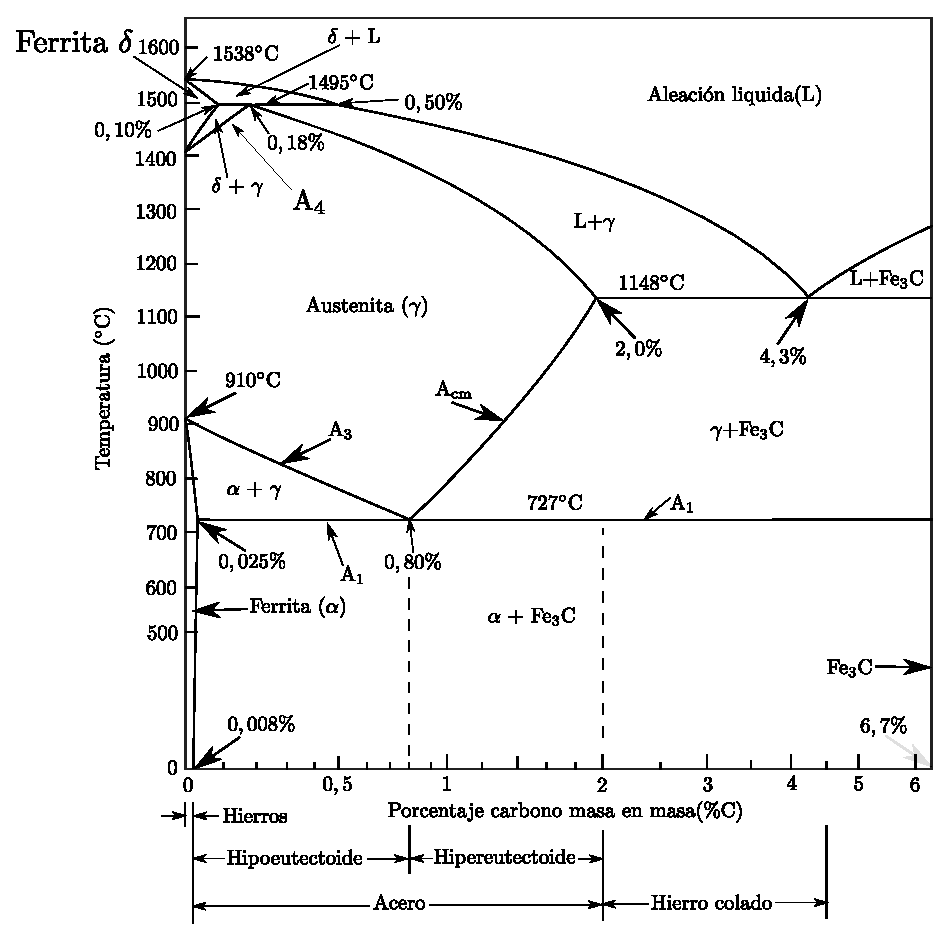
\includegraphics[width=1\textwidth]{fig/diagAceroreal.eps}
    \caption{Diagramas de fases para aceros.}
    \label{fig:diagAceros}
\end{figure}

Fases
\begin{itemize}
    \item Perlita: Morfología laminar, su transformación se favorece con mayor coeficiente de difusión.
    \item Bainita: Morfología con $\alpha$ en listones y carburos discretos
    \item Martensita: Misma composición que austenita pero red cristalina diferente (BCT) y distorsionada. Contiene zonas de austenita.
\end{itemize}



\section{Acero eutectoide}
Se comienza estudiando las transformaciones isotérmicas de la austenita
\begin{figure}[htb!]
    \centering
    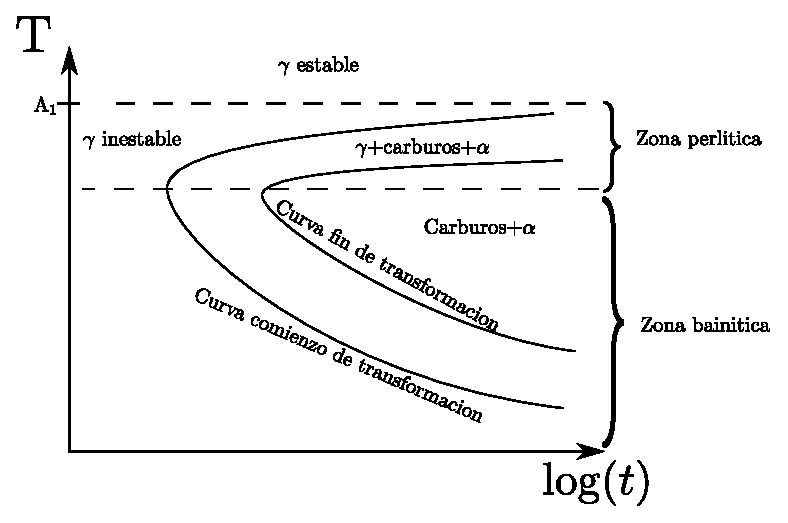
\includegraphics[width=\textwidth]{fig/TTTbasic.eps}
    \caption{Diagrama para transformación isotérmica de la austenita para un acero \textbf{eutectoide}.}
    \label{fig:diagTTTbasico}
\end{figure}

\begin{figure}[htb!]
    \centering
    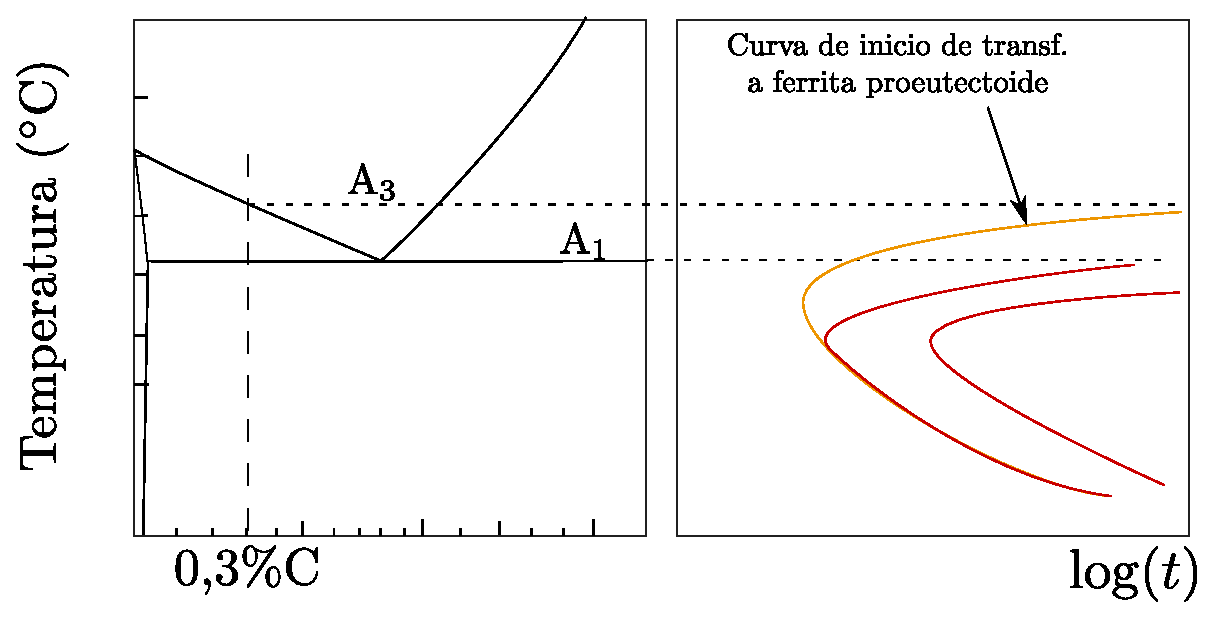
\includegraphics[width=\textwidth]{fig/diagTTThipo.eps}
    \caption{Diagrama para transformación isotérmica de la austenita para un acero \textbf{hipoeutectoide} (0,3\%).}
    \label{fig:diagTTThipo}
\end{figure}

\begin{figure}[htb!]
    \centering
    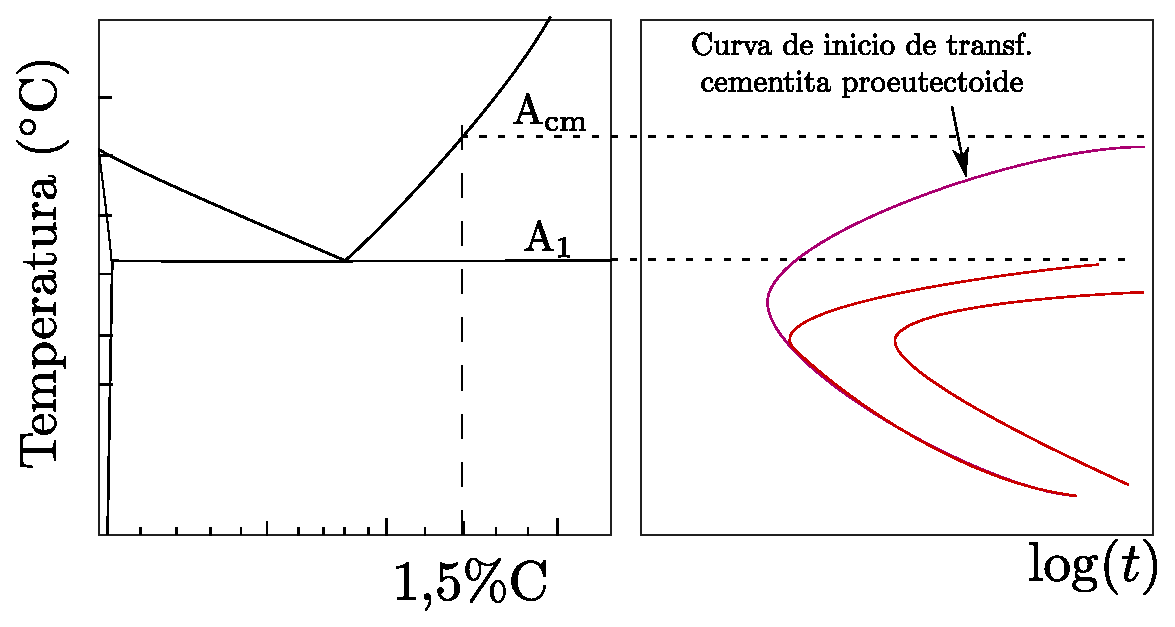
\includegraphics[width=\textwidth]{fig/diagTTThiper.eps}
    \caption{Diagrama para transformación isotérmica de la austenita para un acero \textbf{hipereutectoide} (1,5\%).}
    \label{fig:diagTTThiper}
\end{figure}

La nariz de la figura \ref{fig:diagTTTbasico} se da porque hay competencia entre la \textbf{fuerza impulsora} $\Delta G$ (dominante a bajas temperaturas) y el \textbf{coeficiente de difusión de carbono} $D_c$ (aumenta con temperatura).

Transformación perlítica



\section{Competencia entre G y D}
A temperaturas cercanas a \Aone la difusión domina mientras que a bajas temperaturas hay alta fuerza impulsora debido a que la inestabilidad de la austenita. Hay una temperatura a la cual se complementan y la transformación tiene una velocidad máxima, en la figura \ref{fig:diagTTTbasico} seria la nariz (450 a 600 \grad).

\section{Microconstituyentes}
Los productos de transformación de la austenita que combinan
ferrita y carburos de Fe, así como las fases proeutectoides, se denominan genéricamente \textbf{microconstituyentes} para diferenciarlos de las verdaderas fases que los componen.
\begin{itemize}
    \item Si enfriamos justo por debajo de \Aone~ la fuerza impulsora va ser baja  y van a prevalecer los sitios de nucleacion preferencial (bordes de grano). Comienza a nuclear a la par la ferrita y la cementita cooperativamente formando un microconstituyente con morfologia laminar denominado \textbf{perlita}. Ocurre por arriba de la nariz para subenfriamientos bajos ($<170\grad$).
    \item En cambio, en el rango de temperaturas por debajo de la nariz la ferrita nuclea primero, adopta una morfología de listones, y los carburos ya no son laminares sino discretos con forma de placas más o menos cortas. Por otra parte la transformación en esta zona tiene un mecanismo diferente al aquel que ocurre a altas temperaturas. Los microconstituyentes obtenidos en esta zona se denominan genéricamente \textbf{bainitas} y los hay de varios tipos.
    \item Finalmente, a temperaturas muy bajas ($<$ 350\grad) la austenita subenfriada transforma anisotérmicamente y sin difusión a una fase metaestable denominada martensita.
\end{itemize}


\section{Perlita}
Para generar perlita se requiere un alto coeficiente de difusión de carbono ya que se están generando zonas de muy bajo carbono (ferrita $\alpha$) y zonas de alto carbono (cementita $\cementita$) lo que requiere mucha difusión partiendo de austenita ($\gamma$). Prevalecen los sitios de nucleación preferencial debido a la baja fuerza impulsora $\Delta G$.

El \textbf{espaciado interlaminar} $S$ es el principal parámetro geométrico de la perlita. Tiene gran importancia y determina muchas propiedades. Es la distancia entre laminas contiguas de la misma fase medida perpendicularmente al eje longitudinal de las laminas (básicamente miras la foto de microscopio de electrones y ves cuanto espacio hay entre comienzos de dos laminas de cementita/ferrita). Existe la perlita gruesa ($S\approx 1\si{\micro \meter}$) y perlita fina $S< 0,3\si{\micro \meter}$. A mayor subenfriado menor es $D_c$, menos se puede desplazar el carbono y por ende menor va ser la distancia entre laminas de \cementita~ y $\alpha$.
\begin{equation}\label{eq:StoPerliteStrength}
    R_{p 0,2}, R_{m}, H V \propto S^{-\frac{1}{2}}
\end{equation}

Perlita mas fina trae dureza, resistencia y mayor tensión de fluencia. A su vez es mas difícil de formar, mecanizar etc.

\section{Transformación Martensita}
Cuando la austenita se sobrenfría hasta temperaturas muy bajas se produce una transformación sin difusión de C donde, en un volumen discreto de material, los átomos de Fe experimentan un movimiento cooperativo, pequeño, y casi simultáneo. Esto da por resultado una fase metaestable de igual composición química que la austenita que le dio origen pero con una estructura cristalina diferente. Esta fase se denomina martensita y la transformación se llama transformación martensítica.

En los aceros al C y de baja aleación la martensita tiene estructura tetragonal centrada en el cuerpo (\textit{Body Centered Tetragonal}, BCT). El C, al no poder difundir distorsiona la red y hace que en cambio de nuclearse la fase estable BCC aparezca una fase metaestable BCT.

El movimiento cooperativo genera tensión y deformación en la fase madre. Esta deformación puede causar fisuras y agravar el fenómeno de la fatiga. No hay difusión en la transformación martensítica y se dice que es atérmica (o anisotérmica), es decir que no evoluciona isotérmicamente sino que la fracción de martensita crece en tanto se siga subenfriando la austenita remanente.

$M_s$ es la temperatura de inicio de la transformación martensítica. $M_f,M_{90}$ en principio es la temperatura a la que finaliza dicha transformación. Siempre queda una fracción de austenita muy resistente a la transformación y por ende nunca se puede realmente medir la temperatura de transformación total $M_f$.\footnote{En realidad se define $M_f$ como el límite de 99\% transformación martensítica (definida como fracción de volumen), la temperatura a la cual toda la austenita se convierte a martensita es sustancialmente menor a $M_f$ \cite{gottstein2013physical}.} El subíndice indica la fracción (sobre cien) de martensita producida.

$M_s$ y $M_f$ dependen fuertemente de la composición química de la austenita, con excepción del Cobalto.
\begin{equation}
    M_s=539-423\cdot \% \mathrm{C}-30,4\cdot \% \mathrm{M n}-12,1\cdot \% \mathrm{Cr}-17,7\cdot \% \mathrm{Ni}-7,5\cdot \% \mathrm{Mo}
\end{equation}
como se ve en la ecuación arriba, componentes químicos hacen bajar la temperatura del comienzo de la transformación de austenita. El nitrógeno también tiene un efecto similar al carbono. $M_f$ también baja con aumento de aleantes.

\subsection[Temperatura {\it Md}]{Temperatura $M_d$}
Por debajo de cierta temperatura denominada ($M_d> M_s$), la
deformación plástica aplicada a la austenita provoca la transformación a martensita. El porcentaje de martensita aumenta al aumentar la cantidad de deformación plástica aplicada a la austenita a una determinada temperatura, y al disminuir la temperatura a la cual se aplica la deformación. $M_d$ también depende de la composición química de la austenita y baja al aumentar la cantidad de elementos disueltos en dicha fase. Esta característica cobra gran importancia práctica en el caso de los aceros inoxidables austeníticos. 

\subsection{Estructura Martensítica}
En realidad la estructura BCT de la martensita es una red BCC distorsionada por causa de la presencia del carbono en solución solida sobresaturada. Durante la transformación un eje (denominado \textbf{c}) se achica y otro eje (\textbf{a}) se ensancha, generando una expansión neta dependiente del carbono \footnote{La relación $c/a$ incrementa con la concentración de carbono \cite{gottstein2013physical}.}
\[
\varepsilon_{\Delta V \%} = 4,64-0,54\cdot (\% \mathrm{C})
\]



En martensitas de ``bajo'' carbono (menor a 0,6\%) se presentan los cristales en forma de listones paralelos de ancho 0,2 a 0,5\um~  formando paquetes entre ellos. Esta estructura contiene una gran cantidad de dislocaciones ($10^{11}$ disl/cm$^2$).

En martensitas de ``alto'' carbono (mayor a 0,8\%) y $M_s$ es lo suficientemente baja los cristales adoptan forma lenticular sin formación de paquetes. El plano de habito de estas estructuras puede ser el $\{225 \}_\gamma$ o el $\{259 \}_\gamma$ dependiendo del porcentaje de carbono. Debido a esto se pueden tener dos placas adyacentes con planos diferentes dándole un aspecto caótico a la estructura y generando microfisuras.

La dureza de la martensita se debe a los siguientes factores
\begin{itemize}
    \item \hl{Endurecimiento por solución solida: intersticial del carbono}
    \item \hl{Interacción dislocaciones - carbono segregado. Una vez cristalizada la martensita el carbono se puede segregar a sitios donde baja la energía del sistema. Las dislocaciones son lugares preferenciales (anclaje = dureza agregada)}
    \item Interacción entre dislocaciones
    \item Gran cantidad de bordes de grano (bajo y alto ángulo)
    \item Endurecimiento por solución solida sustitucional
\end{itemize}

\textbf{La dureza de la martensita depende fuertemente del \%C de la austenita que le dio origen. El efecto del C es tan preponderante que, en términos prácticos, ningún otro factor tiene importancia en esta propiedad.}

Como es de esperar, un material tan duro es tambien frágil, y la martensita no es ninguna excepción. A mayor \%C la martensita es menos dúctil y menos tenaz. Se puede hacer un \textbf{revenido} para producir transformaciones de fase que modifican la estructura de la martensita, transformándola en una estructura de ferrita y carburos dispersos (denominada genéricamente \textbf{martensita revenida}). La martensita no comienza su transformación a temperatura $M_s$, es necesario llevarla a $A_s$ (temperatura de comienzo de austenización) \cite{gottstein2013physical}.

\section{Bainita}

Cuando el subenfriamiento de la austenita supera los 150-170\grad~ la transformación perlítica se hace lenta y comienza a dominar $\Delta G$. Ambas cosas dan origen a una transformación que combina algunos aspectos de la transformación martensítica y otros de la perlítica. Este tipo de transformación se denomina bainítica y los microconstituyentes que se producen se denominan genéricamente bainitas.

Los tipos de bainitas mas estudiados son la bainita \textbf{superior} y \textbf{inferior}.

\begin{itemize}
    \item Bainita superior: Entre la nariz y una temperatura dependiente del \%C aparece.
    \item Bainita inferior: Por debajo de dicha temperatura se produce la bainita inferior de distinta morfología a la superior.
\end{itemize}

A partir de una limite superior, la temperatura $B_s$, ya no se forma Bainita.

\[
B_{S}\left(^{\circ} C\right)\approx550-270 \cdot\%\mathrm{C}-90\cdot\%\mathrm{Mn}-37 \cdot\%\mathrm{Ni}-70 \cdot\%\mathrm{Cr}-83\cdot\%\mathrm{Mo}
\]

\subsection{Bainita superior}
Comienza con crecimiento de listones de ferrita de 0,02\%C en los borde de granos austeníticos. Esto deja la austenita del entorno del listón rica en carbono, eventualmente precipitando como carburo en forma de placas finas entre los listones de ferrita y los borde de grano de la antigua austenita.

Estos listones de ferrita contienen una alta densidad de dislocaciones esto se debe a que el mecanismo de transformación involucra un movimiento cooperativo de átomos.
\begin{itemize}
    \item Fácil de nuclear fisuras entre listones y \cementita
    \item Es deseable que la bainita superior sea de bajo carbono para reducir cantidad de laminas de \cementita y mejorar la tenacidad.
\end{itemize}



\subsection{Bainita inferior}
Como la temperatura es mas baja el carbono no logra difundir bien. En consecuencia precipitan carburos dentro de los listones de ferrita dejando atrás laminas a 60 grados del eje del listón. Dependiendo de la composición química del acero los carburos pueden ser \cementita~ o bien el carburo de transición $\varepsilon$.
\begin{itemize}
    \item Es mas difícil de nuclear fisuras u hoyuelos en las partículas finas de este material
    \item Es mas resistente y tenaz que la bainita superior
    \item \textbf{Austempering} tratamiento térmico isotérmico diseñado para obtener bainita inferior debido a sus excelentes propiedades 
\end{itemize}


\subsection{Propiedades mecánicas}
La resistencia mecánica y dureza de las bainitas crecen a medida que baja la temperatura de transformación.

\begin{figure}[htb!]
    \centering
    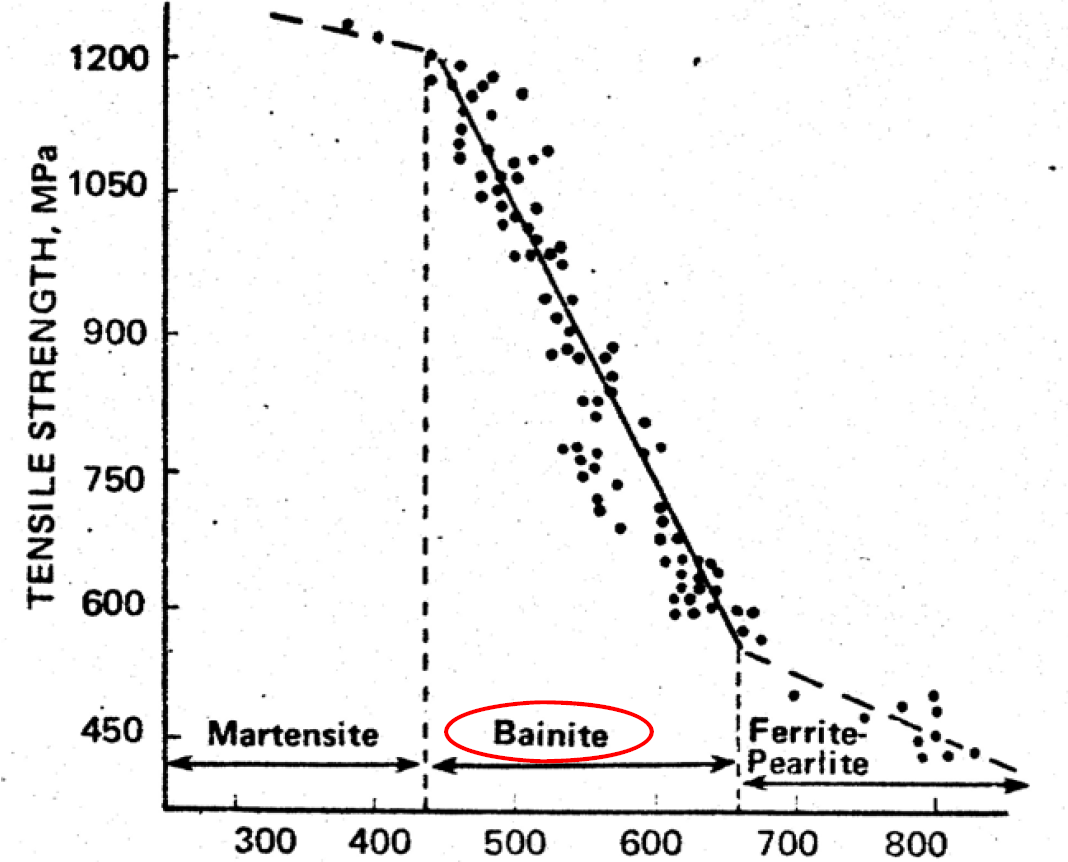
\includegraphics[width=0.7\textwidth]{fig/RmVsBainitaMartensita.PNG}
    \caption{Efecto de 50\% de la temperatura transformación sobre la resistencia a la tracción de aceros bainíticos.}
    \label{fig:RmVsBainitaMartensita}
\end{figure}

Las curvas TTT de la transformación total son en realidad la envolvente de la superposición de las curvas de cada una de las transformaciones individuales. Los aleantes pueden separar estas narices y pronunciarlas mas.

En general a menor temperatura de transformacion la estructura resultante de la austenita es mas fina y por ende resulta ser mas resistente mecánicamente y dura. La excepcion de esta regla es para la perlita fina y bainita superior. \hl{La perlita fina resulta ser mas dura y resistente que bainita superior} a pesar de tener una temperatura de transformacion superior. Esto se debe a que la estructura de la bainita superior es mas gruesa que la estructura de la perlita fina.

\begin{figure}[htb!]
    \centering
    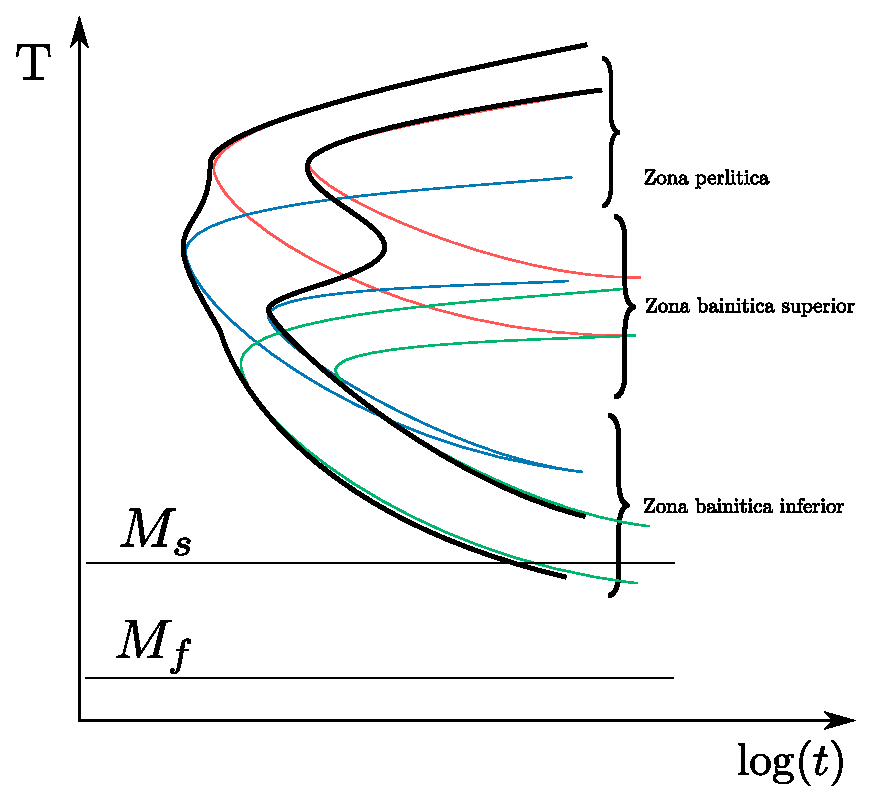
\includegraphics[width=0.7\textwidth]{fig/TTTsuperpuesta.eps}
    \caption{Superposición de curvas perlíticas (rojo) y bainíticas superior (azul) e inferior (verde).}
    \label{fig:TTTsuperpuestas}
\end{figure}

\section[Transformación de la austenita]{Variables que inciden en transformación de la austenita}
Dos variables que inciden en la cinética de estas transformaciones
\begin{itemize}
    \item El tamaño del grano austenítico
    \item La composición química de la austenita que se transforma.
\end{itemize}

Los borde de granos son los sitios de nucleación preferencial para las transformaciones perlítica y bainítica así como para la aparición de las fases proeutectoides ferrita y cementita. Por ende:
\begin{itemize}
    \item Mayor tamaño de grano \goright
    \item[\goright] Menor superficie total de bordes de granos \goright
    \item[\goright] Menor sitios de nucleación \goright
    \item[\goright] Transformaciones comienzan a mayores tiempos
\end{itemize}
\textbf{lo que implica que con mayor tamaño de grano las curvas se mueven a la derecha.}

La composición química juega un rol importante en el efecto sobre $\Delta G$ y $D_c$. Los elementos \textbf{gamágenos} hacen descender la energía libre de la austenita lo que reduce tanto la velocidad de nucleación como la de crecimiento. Los elementos alfágenos hacen subir la fuerza impulsora y en principio deberían acelerar las transformaciones, pero \hl{hacen exactamente lo contrario}.

Porqué sucede esto? En las palabras del profesor (resumidas): Durante la nucleación de ferrita en los borde de grano ocurre que los elementos \textbf{alfágenos} necesitan repartirse hacia la ferrita y los \textbf{gamágenos} necesitan concentrarse en la austenita. Ambos tienen un coeficiente de difusión mucho menor al del carbono y por eso se retrasan las transformaciones de fase.

Además! Los alfágenos son \textbf{formadores de carburos} lo que significa que se tienen que repartir hacia los mismos para que precipiten. Esto también retrasa las transformaciones que involucran precipitación de carburos. 

Algunos elementos simplemente retrasan la difusión del carbono, lo que también retrasa las transformaciones.

Efectos de elementos alfágenos:
\begin{itemize}
    \item Suben \Aone y \Athree (estabilización de ferrita [$\alpha$])
    \item Bajan \Bs, separando las curvas perlíticas y bainíticas
    \item Retrasan más la transformación ferrítica y perlítica que la bainítica. El Molibdeno acelera débilmente la transformación bainítica
    \item El Boro en diminutas cantidades (60ppm) provoca un fuerte retraso en la nucleación de la ferrita proeutectoide. De aquí surgen aceros de alta templabilidad.
\end{itemize}

Efectos de elementos gamágenos:
\begin{itemize}
    \item Bajan temperaturas \Aone, \Athree, \Bs y $M_s$
    \item Retrasan ambas transformaciones (perlita, bainita)
\end{itemize}

\section{Curvas CCT}
\textit{Continuous Cooling Transformation} son curvas representativas de las fases obtenidas a velocidad de enfriamiento constante. Cuando el enfriamiento es continuo desde el campo estable de $\gamma$, el tiempo de comienzo de la transformación no coincide con el que dice la curva TTT. Es porque la austenita pasa por un rango de T donde los periodos de incubación son grandes, de esta forma ``retrasando'' las curvas respecto las TTT.

\begin{figure}[htb!]
    \centering
    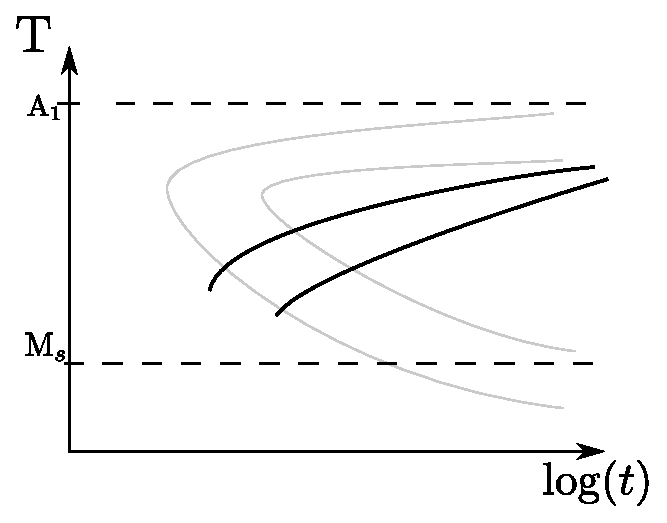
\includegraphics[width=0.8\textwidth]{fig/CCTeutect.eps}
    \caption{Curvas de enfriamiento continuo (CCT) para un acero \textbf{eutectoide}. CCT en negro, curvas TTT en gris claro.}
    \label{fig:CCTeutect}
\end{figure}

\subsection{CCT para un acero hipoeutectoide}
Las curvas de enfriamiento para un acero \textbf{hipoeutectoide} de la figura \ref{fig:CCThipo} pueden ceder las siguientes estructuras y microconstituyentes:\footnote{Tener en cuenta que las curvas rojas de la figura \ref{fig:CCThipo} se dibujan hasta donde haya austenita sin trasformar, es decir, el final de la curva esta donde $\gamma=0\%$.}


\begin{itemize}
    \item[Ciclo 1] Se obtiene ferrita de grano grueso y perlita gruesa en fracciones cercanas al equilibrio
    \item[Ciclo 2] Ferrita de grano mas fino que en el ciclo 1 y perlita fina. Perlita es diluida en ferrita que se encuentra presente en cantidades mayores a la de equilibrio. 
    \item[Ciclo 3] Ferrita, bainita y una fracción de Martensita que sale de la austenita que no se transformo al llegar a $M_s$ \footnote{La curva $M_s$ no es constante para todos los aceros. Si se tiene un acero hipereutectoide, al comenzar a formar bainita la concentración de carbono en la austenita sin transformar va aumentar, reduciendo asi $M_s$ a menor velocidad de transformación por ser un elemento gamágeno.}
    \item[Ciclo 4] Mínima velocidad de transformacion para lograr 100\% de martensita denominada \hl{Velocidad Critica de Temple}
\end{itemize}

\begin{figure}[htb!]
    \centering
    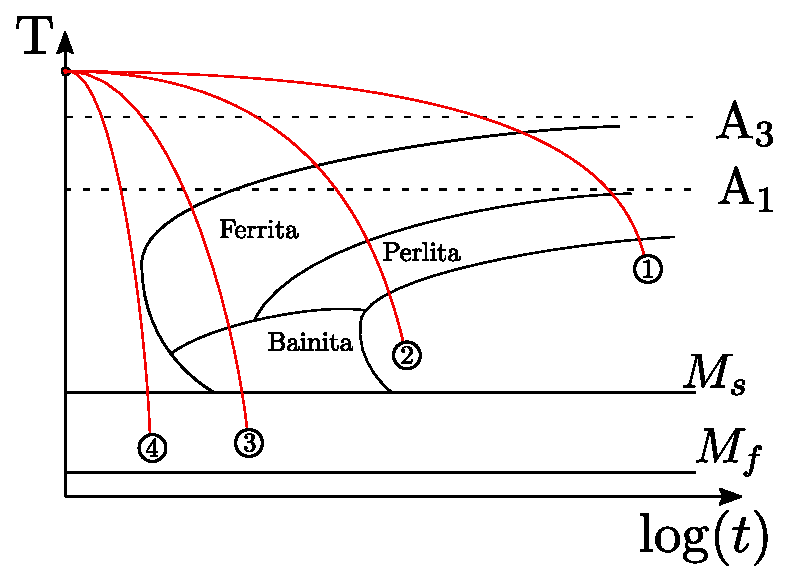
\includegraphics[width=0.7\textwidth]{fig/CCThipo.eps}
    \caption{Curvas de enfriamiento continuo (CCT) para un acero \textbf{hipoeutectoide}.}
    \label{fig:CCThipo}
\end{figure}

NOTA: La curva $M_s$ baja después de un tiempo dado!


\subsection{Variación de propiedades mecánicas con la velocidad de enfriamiento}
Aumentando la velocidad de enfriamiento de la austenita, las transformaciones ocurren en un rango de temperaturas más bajas, logrando microconstituyentes más finos que conlleva con un aumento de dureza y resistencia a la tracción. 

Las estructuras que surgen de un enfriamiento continuo son más complejas que las de transformaciones isotérmicas ya que al pasar por un rango más amplio de temperaturas de transformación se pueden obtener mezclas muy variadas de los microconstituyentes.
% !TeX spellcheck = es_ES
% !TeX root = ../metalurgy.tex
\part{Tratamientos térmicos}
Un tratamiento térmico (TT) es un ciclo térmico aplicado a un metal con el objeto de obtener una cierta combinación de propiedades, también puede usarse para relevar tensiones residuales. La modificación de las propiedades tiene una profunda relación con las transformaciones de fase que ocurren en el metal a causa del ciclo térmico.

Clasificación de TT de aceros:
\begin{itemize}
    \item Sin cambio de composición química
    \begin{itemize}
        \item Volumétrico
        \item Local
    \end{itemize}
    \item Termoquímicos
    \item Hipercrítico $T>$\Athree~
    \item Intercrítico $\Aone<T<\Athree$ o \Acm~
    \item Subcrítico $T<$ \Aone~
\end{itemize}



\section{Austenización}
No es un tratamiento en sí, es la primer etapa de cualquier tratamiento térmico hipercrítico (TTH). Una vez llegado a la temperatura \Athree{} comienza el lento proceso de austenización. Se acelera la transformación con el aumento de la temperatura, pero hay factores que impiden utilizar temperaturas demasiado altas.

\begin{itemize}
    \item \textbf{Costo} aumenta más fuertemente con la temperatura que con el tiempo. (Energía y vida útil de instrumentos)
    \item \textbf{Tamaño de grano austenítico crece} al aumentar temperatura. Trae problemas en propiedades finales y fisuración en TT posteriores
    \item \textbf{Oxidación} aumenta y se propaga al interior del material. Limita uso de materiales de pequeño espesor. Se puede usar una atmósfera protectora.
    \item \textbf{Sobrecalentamiento y quemado} a altas temperaturas (1100\grad). Suele traer problemas para conformado en caliente posterior o para tratamientos de aceros de alta aleación
\end{itemize}

La temperatura a la cual se decide austenizar se llama, apropiadamente, \textbf{temperatura de austenización} ($T_A$) siendo esta mayor a \Athree{} o \Acm{}. $T_A$ surge de un compromiso entre la necesidad de disminuir el tiempo del austenizado y la de evitar los fenómenos antes mencionados. 

$T_A$ varía para cada acero y proceso dependiendo principalmente de
\begin{itemize}
    \item Composición química
    \begin{itemize}
    	\item Para aceros de alta aleaci\'on la cantidad de alf\'agenos aumenta \Athree. $T_A$ puede llegar a los 1300\grad~
    \end{itemize}
    \item Tipo de TT que se aplicara posterior al austenizado
\end{itemize}

El tiempo de austenización depende de
\begin{itemize}
    \item \textbf{Sección máxima} de la pieza ya que el núcleo de la pieza va tardar en tomar temperatura y austenizar. También influye el horno (potencia, capacidad, tipo)
    \item \textbf{Temperatura $T_A$.} Aumenta velocidad de austenización con su aumento
    \item \textbf{Microestructura}: Si se tiene carburos gruesos, zonas segregadas, o una alta aleación estos tardaran en disolverse
\end{itemize}

Cabe destacar que la velocidad de calentamiento no es factor importante para aceros de baja aleación. Estos se pueden cargar en el horno a $T_A$. Para aceros de alta aleación hay varias razones para controlar la velocidad de calentamiento.
\begin{enumerate}
    \item \textbf{Evitar tensiones térmicas.} Aceros de alta aleación tienen mayor coeficiente de dilatación térmica
    \item \textbf{$T_A$ mayor.} Debido a la gran cantidad de alfágenos
    \item \textbf{Mayor \% carbono.} Mayor fragilidad y riesgo de fisuración
    \item \textbf{Geometrías complejas.} Influye en concentración de tensiones térmicas
\end{enumerate}

{\bf Resumiendo}: El objetivo del austenizado es obtener, en el menor tiempo posible, una austenita químicamente homogénea, de tamaño de grano fino y homogéneo, minimizando la modificación de la composición química de la superficie, y reduciendo la distorsión y riesgo de fisuración que pudiera producirse durante el calentamiento o durante la mantención a la temperatura de austenización. 

Es una etapa fundamental para cualquier tratamiento hipercrítico, en especial para aquellos que buscan endurecer el acero. El resultado del tratamiento térmico depende en gran parte de una correcta austenización.

\section{Tratamientos hipercríticos}
Los tratamientos hipercr\'iticos llevan el acero a una temperatura sobre \Athree~ para lograr austenizaci\'on de una gran parte del acero.
\subsection[Recocido de regeneración]{Recocido de regeneración (Full annealing)}
Consiste en llevar el acero a $T_A$\footnote{Para aceros hipoeutectoides suele estar a 20 a 40\grad~ sobre \Athree~} y mantenerlo ahí un tiempo adecuado para asegurar la homogeneidad de la austenita y luego un enfriamiento lento en horno (costoso económicamente) de alrededor de 5 a 50\grad{}/h. Para un acero hipoeutectoide el recocido de regeneraci\'on ser\'ia el camino 1 de la figura \ref{fig:CCThipo}.

\begin{figure}[htb!]
\centering
\begin{subfigure}{0.4\textwidth}
    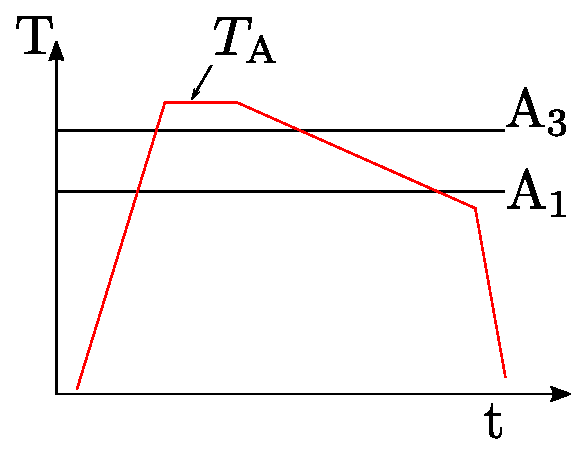
\includegraphics[width=\linewidth]{fig/TTrecoreg.eps}
    \caption{\textbf{Hipercrítico}.}
    \label{fig:TTrecoreg}
\end{subfigure}
\begin{subfigure}{0.4\textwidth}
    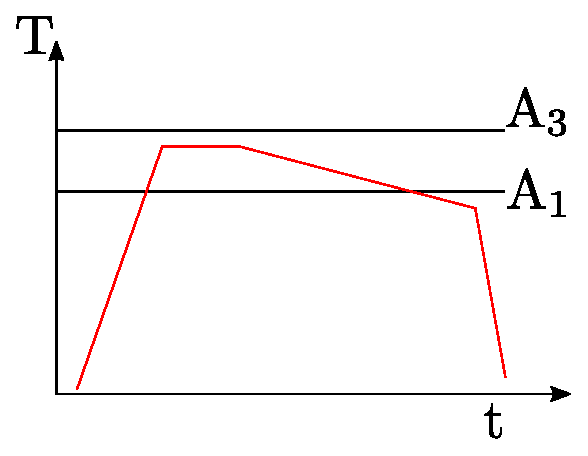
\includegraphics[width=\linewidth]{fig/TTrecoreghiper.eps}
    \caption{\textbf{Intercrítico} para aceros hipereutectoides.}
    \label{fig:TTrecoreghiper}
\end{subfigure}
\caption{TT Recocido de regeneración.}
\end{figure}



Se obtiene una perlita gruesa que conlleva una dureza baja. Si es lo suficientemente lento el enfriamiento se puede obtener perlita parcialmente esferoidizada.

Objetivos:
\begin{itemize}
    \item Reblandecer el acero
    \begin{itemize}
        \item Estructuras de ferrita proeutectoide de tamaño de grano grueso y perlita gruesa, implica mejor formabilidad y maquinabilidad a costo de dureza
    \end{itemize}
    \item Llegar a estructura favorable para el mecanizado y deformación en frió
    \item Obtener otras propiedades finales especificas
    \begin{itemize}
        \item Aplicaciones en industria bulonera para mejorar proceso de recalcado y laminación de roscas
    \end{itemize}
\end{itemize}

El \textbf{recocido de regeneración isotérmico} consiste en realizar la transformación de la austenita a una temperatura constante y relativamente cercana a la de equilibrio. Es mas rápida pero puede dejar el acero con una dureza mayor y requiere de un horno de sales.

\begin{figure}[htb!]
    \centering
    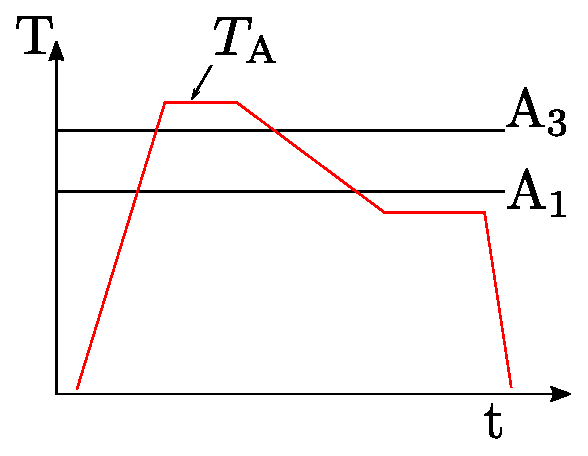
\includegraphics[width=0.5\textwidth]{fig/TTrecoregiso.eps}
    \caption{Recocido de regeneración isotérmico.}
    \label{fig:TTTrecocidoregeneracionisotermico}
\end{figure}

En el caso de los aceros \textbf{hipereutectoides} el tratamiento es \hl{intercrítico} para evitar precipitación de laminas de \cementita~ en los bordes de grano de la austenita.

\textbf{Resumiendo:} el recocido de regeneración es un tratamiento largo y costoso que deja al acero en un estado de baja dureza y alta ductilidad. En aceros de medio y alto C esto es muy conveniente para reducir los costos del conformado plástico en frío y/o del mecanizado. Menos frecuentemente se puede usar para lograr propiedades finales.

\subsection{Normalizado}
Similarmente al recocido, en el \textbf{normalizado} se calienta el acero hasta $T_A$\footnote{Temperatura unos 50 a 80\grad~ sobre \Athree~} y se mantiene para asegurar austenita homogénea y finalmente se \textbf{enfría a aire calmo}\footnote{Velocidad entre 40 a 200\grad{}/min}. Si se busca obtener martensita se denomina \textbf{temple al aire}. El normalizado puede ser tanto un tratamiento intermedio como también un tratamiento final.

\begin{figure}[htb!]
    \centering
    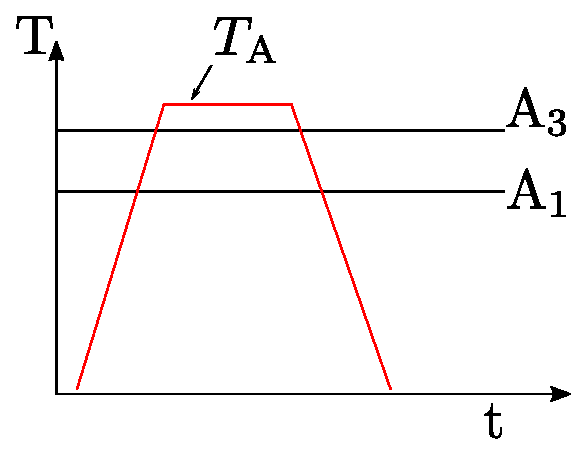
\includegraphics[width=0.5\textwidth]{fig/TTnorm.eps}
    \caption{Normalizado.}
    \label{fig:TTnorm}
\end{figure}

Objetivos:
\begin{itemize}
    \item Homogeneización química y estructural
    \item Refinamiento de tamaño de grano ferritico y de los carburos
    \item Preparar mejor al acero para un tratamiento posterior (dos puntos anteriores)
    \item Mejorar maquinabilidad en aceros bajo carbono
    \item lograr propiedades mecánicas especificas para el servicio
\end{itemize}

La estructura resultante depende de la composición del acero y tamaño de la pieza. En aceros al C y muchos de baja aleación se obtiene ferrita proeutectoide de tamaño más fino que en el recocido y en menor proporción. El resto de la estructura es perlita más fina y en mayor proporción de lo que indica el diagrama de equilibrio. En aceros con transformaciones más lentas pueden aparecer combinaciones de otras fases incluyendo la bainita y martensita.

El normalizado se aplica típicamente a piezas coladas y forjadas en caliente para refinar la estructura de solidificación. Para aceros de bajo \%C se vé un aumento en la maquinabilidad.
\section{Tratamientos subcríticos}

\subsection{Recocido de relevamiento de tensiones}
Consiste en calentar el acero hasta una $T<$\Aone{} y mantenerla un tiempo adecuado para disminuir tensiones residuales y luego enfriar lentamente\footnote{5 a 10\grad/h}.

Objetivos:
\begin{itemize}
    \item Disminuir tensiones residuales
    \item Evitar fenómenos de \textbf{rotura diferida} causados por el hidrógeno o bien algún tipo de corrosión bajo tensión.
    \item Aumentar \textbf{estabilidad dimensional}
\end{itemize}

\subsection{Recocido de globulización}
Consiste en calentar al acero hasta una $T$ por debajo a \Aone~ y mantenerla un tiempo adecuado. Microestructuralmente se busca globulizar los carburos laminares de la perlita. Es usado solo en aceros de más de 0,4\%C y principalmente en esos que deban ser sometidos a operaciones de conformado muy severas. Para aceros hipereutectoides, este es el tratamiento más común ya que aumenta la maquinabilidad en aceros de baja aleación.

\begin{figure}[htb!]
    \centering
    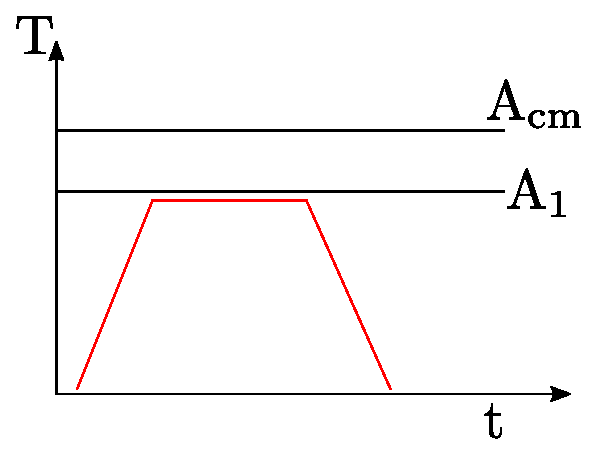
\includegraphics[width=0.5\textwidth]{fig/TTglob.eps}
    \caption{Recocido de globulización \textbf{subcrítico}.}
    \label{fig:TTglob}
\end{figure}

La fuerza impulsora para la esferoidización es la energía de interfaz. Es muy baja y por ende se requiere largos tiempos. Cuanto menor es el espaciado interlaminar de la perlita, mas rápido es el proceso. Se puede también acelerar el proceso con deformación plástica previa.

Clasificación de estos recocidos, incluyendo las versiones que no son subcríticas:
\begin{itemize}
    \item Subcrítico $T\approx\Aone-50\grad$. Se requiere mucho tiempo. Puede ser acelerado con deformación plástica previa a costo de deformar mi pieza. Es el que se toma en el parcial.
    \item intercrítico $T\approx\Aone+50\grad$. Más corto pero se requiere un estricto control de temperatura y en la velocidad de enfriamiento
    \item Oscilante $T\in\{\Aone-50\grad;\,\Aone+50\grad \}$. Misma ventajas/desventajas que intercrítico.    
\end{itemize}

El recocido de globulización

\section{Temple}

Consiste en austenizar al acero totalmente o parcialmente\footnote{Para acero hipoeutectoides varia entre 40 a 60\grad~ sobre \Athree.} y luego enfriarlo suficientemente rápido para obtener una fracción significativa de martensita (en general no menos de 50\%). 

Clasificación de Temples
\begin{itemize}
    \item Superficial
    \begin{itemize}
        \item Inducción
        \item Llama
    \end{itemize}
    \item Local
    \item Volumétrico
\end{itemize}
Clasificación por método
\begin{itemize}
    \item Por inmersión
    \item Por aspersión o neblina
    \item En matriz metálica refrigerada
\end{itemize}

La \textbf{velocidad critica} es la mínima velocidad de enfriamiento para asegurar 100\% martensita. Es un indicador de templabilidad y esta relacionada con la posición de la nariz de la curva CCT.

El \textbf{efecto de masa} se le dice a la variación de la velocidad de enfriamiento entre distintos puntos de una pieza causada por su inercia térmica. El efecto es mayor a medida que aumenta el tamaño de la pieza.

\subsection[Severidad de temple]{Severidad de temple ($H$)}
Propiedad del medio de temple que indica su capacidad para extraer el calor desde la superficie de la pieza. Una severidad infinita baja instantáneamente la temperatura de la pieza hasta la del baño de temple. La severidad de temple $H$ se mide experimentalmente y depende fuertemente de la composición del medio de temple (que determina sus propiedades térmicas y otras propiedades físicas como la presión de vapor, densidad, viscosidad, etc), de su temperatura y de su grado de agitación. 


\begin{table}[htb!]
\centering
\begin{tabular}{l|l|l|l|l}
\hline
\multicolumn{1}{c|}{\multirow{2}{*}{Agitación}} & \multicolumn{4}{c}{Medio}            \\ \cline{2-5} 
\multicolumn{1}{c|}{}                           & Aire & Aceite    & Agua    & Salmuera \\ \hline
Ninguna                                         & 0,02 & 0,25-0,30 & 0,9-1,0 & 2        \\
Moderada                                        & -    & 0,3-0,4   & 1,0-1,3 & 2-2,2    \\
Acentuada                                       & -    & 0,4-0,5   & 1,4-1,5 & -        \\
Fuerte                                          & 0,05 & 0,5-0,8   & 1,6-2,0 & -        \\
Violenta                                        & -    & 0,8-1,1   & 4       & 5        \\ \hline
\end{tabular}
\caption{Severidad de Temple ($H$)}
\label{tab:severidadTemple}
\end{table}

Lo mejor que hay de medio de temple es salmuera seguido de agua y aceites. Agua a 20 \grad{} tiene un $H=1$ por definición. Los aceites tienen la ventaja de tener velocidad baja en la etapa \ref{item:etapaCEnfriamiento} (secci\'on \ref{ssec:enfriamientoEnMedio}), esto evita fisuras. 

Lo mas deseable es enfriamiento rápido en las primeras etapas y un enfriamiento lento en la etapa \ref{item:etapaCEnfriamiento} para no fisurar la pieza. Se puede cambiar el medio de temple de agua a aceite terminado las primeras etapas pero esto requiere un maestro templador y no se puede hacer de forma industrializada.

La agitación contribuye a la severidad del temple y reduce  duración de la etapa A. También aumenta la velocidad de enfriamiento de la etapa \ref{item:etapaBEnfriamiento} pues ayuda desprender las burbujas de vapor. Genera convección forzada en etapa \ref{item:etapaCEnfriamiento}  aumentando enfriamiento.

Elección de severidad de temple para lograr una cierta dureza $\HB_{\mathrm{deseada}}$
\begin{itemize}
    \item Mayor templabilidad del acero \goright Menor severidad
    \item Si la pieza es grande o el acero no puede llegar a $\HB_{\mathrm{deseada}}$ aun con la mayor severidad de temple posible se deberá usar un acero mas templable
    \item Es necesario evaluar la aplicabilidad de la severidad para disminuir el riesgo de fisuración ya que el calculo de templabilidad no garantiza que se pueda alcanzar $\HB_{\mathrm{deseada}}$ sin fisurar.
\end{itemize}
\textbf{Conclusión:} Necesito alta \textbf{templabilidad} para la mayoría de los casos!

\subsection{Templabilidad}
La \textbf{templabilidad} es la capacidad de una aleación ferrosa (acero o fundición) para obtener martensita a partir de la austenita cuando esta se enfría en condiciones bien definidas. Está relacionada con la cinética de las transformaciones con difusión de la austenita cuando esta es enfriada y por lo tanto con la posición y forma de las curvas de transformación CCT del acero. \hl{Es una propiedad intrínseca y no depende de el tamaño de la pieza o la velocidad de enfriamiento.}
\begin{figure}[htb!]
    \centering
    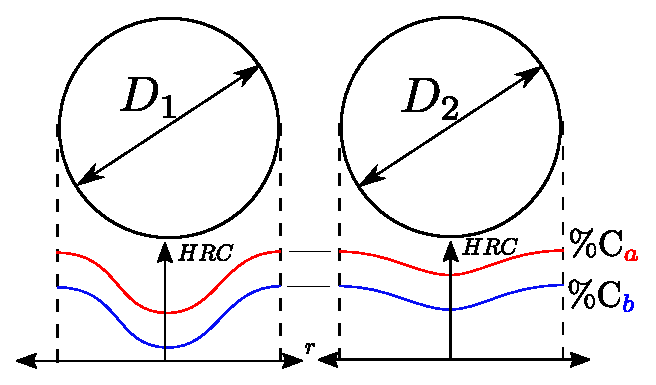
\includegraphics[width=0.6\textwidth]{fig/Templabilidad.eps}
    \caption{Dureza en función de posición $r$ donde $D_1 = D_2$. La probeta 1 es un acero de baja aleación y la probeta 2 es un acero de alta aleación (más templable). Porcentaje carbono ${\color{red} a}> {\color{blue} b}$. }
    \label{fig:templabilidad}
\end{figure}
Los siguientes factores controlan la templabilidad
\begin{enumerate}
    \item Aleantes (con la excepción del cobalto)
    \begin{itemize}
        \item Retrasan las transformaciones con difusión (perlítica y bainítica) aumentando así la templabilidad
        \item Efecto sinérgico entre aleantes significa que conviene mezclar pequeñas cantidades de varios aleantes
    \end{itemize}
    \item Tamaño de grano
    \begin{itemize}
        \item A mayor tamaño de grano se tiene mayor templabilidad
        \item No se usa para aumentar la templabilidad pues conlleva un deterioro en las propiedades finales
    \end{itemize}
    \item Presencia de otras fases
    \begin{itemize}
        \item Presencia de otras fases aumenta sitios de nucleación y acelera transformaciones con difusión
        \item Estas fases pueden retener aleantes
    \end{itemize}
\end{enumerate}


\setcounter{footnote}{0}

\subsection[Diámetro crítico]{Diámetro crítico ($D_0$)}
 Se define como el máximo diámetro en el que puede obtenerse 50\% martensita en el centro cuando se lo enfría con un medio de temple bien definido. Para un $D<D_0$ se tendrá menos de 50\% martensita en el centro.

\textbf{Diámetro critico ideal} $D_{I}$: El diámetro para el cual se obtiene 50\% martensita en el centro de la pieza con \textit{severidad de temple infinita} $H=\infty$, es decir que la superficie de la pieza en contacto con el medio de temple toma la temperatura del medio en tiempo nulo. $D_{I}>D_0$

\subsubsection{Ensayo de Jominy (End-Quench)}
\hl{Se templa una probeta (previamente austenizada) con un chorro de agua en desde un extremo}. Luego se rectifica la probeta \textbf{longitudinalmente} y se mide la dureza en varios puntos, cada uno a una distancia $d_j$\footnote{Se suele denominar distancia de Jominy.} del extremo templado. Las condiciones que afectan la velocidad de enfriamiento también están estandarizadas: velocidad y temperatura del agua, diámetro del caño que conduce el agua hacia el extremo que se templará, y distancia entre este caño y el extremo de la probeta.

\begin{figure}[htb!]
    \centering
    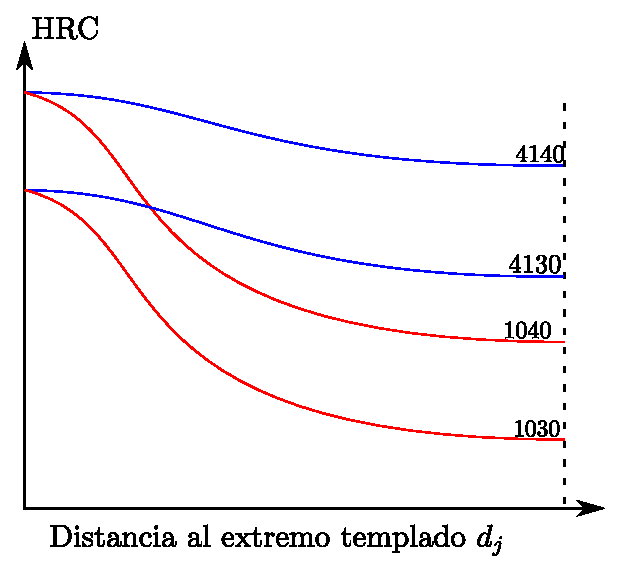
\includegraphics[width=0.7\textwidth]{fig/jominy.eps}
    \caption{Curvas de Jominy para aceros de alta aleación(en {\color{blue} azul}) y para aceros al carbono(en {\color{red} rojo}). A mayor porcentaje de carbono hay mayor dureza en el extremo templado.}
    \label{fig:jominy}
\end{figure}

La ventaja del temple desde un extremo respecto de un temple por inmersión es que se logra un rango de velocidades de enfriamiento muy amplio en una probeta relativamente pequeña. Mientras que el extremo templado se enfría muy enérgicamente ($>200$ \grad/s), el otro extremo sufre algo parecido a un tratamiento de normalizado. Entre estos dos extremos se logran diferentes velocidades de enfriamiento y por lo tanto distintas estructuras y durezas.

\textbf{La curva de Jominy}: Agregar carbono aumenta dureza del extremo templado. Mayor templabilidad achata la curva

\textbf{Templabilidad garantizada:} Cuando la curva Jominy de un acero presenta una dureza dentro de los limites preestablecidos se dice que es un \textbf{acero de templabilidad garantizada} y se le agrega un sufijo a la designación AISI/SAE. Ejemplo: ``SAE 1340 H'' 


Se prefiere una alta templabilidad en los siguientes casos
\begin{itemize}
    \item En piezas de sección grande debido al efecto masa que no permite alcanzar velocidades rápidas en el núcleo de la pieza
    \item Piezas de geometría compleja donde existe alto riesgo de fisuraci\'on. La templabilidad reduce el riesgo de fisuración
\end{itemize}

Los cálculos de templabilidad permiten determinar 

\begin{itemize}
    \item 
\end{itemize}



\subsection{Enfriamiento en medio volátil}\label{ssec:enfriamientoEnMedio}
Se distinguen en tres etapas
\begin{enumerate}[label=(\Alph*)] \label{enum:etapasTemple}
    \item A temperatura de pieza alta se forma una envuelta de vapor sobre la superficie de la pieza. Sin agitación esta envuelta es estable y aísla al metal del liquido. El rango de temperaturas en la que ocurre esta etapa se solapa con aquel en que deben evitarse las transformaciones con difusión para poder obtener martensita, por lo tanto es importante reducir la duración de esta etapa. Se puede reducir esta etapa agregando componentes que reduzcan la presión de vapor (para agua hidróxidos y sales)\label{item:etapaAEnfriamiento}
    \item Una vez reducida la temperatura lo suficiente la envuelta se desestabiliza y se pasa a una etapa donde el calor se extrae principalmente como calor de vaporización. \label{item:etapaBEnfriamiento}
    \item cuando la temperatura baja lo suficiente, se detiene la formación de burbujas de vapor y el calor se extrae por conducción y convección del líquido. La velocidad de enfriamiento vuelve a ser baja. \label{item:etapaCEnfriamiento}
\end{enumerate}



\subsection{Origen de tensiones térmicas durante el temple}
Los conceptos básicos son que la transformación de austenita a martensita es una expansión mientras que el enfriamiento es una contracción. 
\begin{enumerate}
    \item Durante el enfriado ($T_{\mathrm{superficie}}>M_s$) la periferia se \textbf{contrae} mas que el centro ocasionando pequeñas tensiones que se relajan por deformación plástica debido a la alta temperatura. 
    \item Eventualmente la temperatura cae lo suficiente como para que la superficie comience a transformarse ($T_{\mathrm{superficie}}<M_s$) y trata de \textbf{expandirse} pero es restringida por el núcleo generando tensiones de compresión en la periferia y tracción en el núcleo. Aun se pueden relajar las tensiones por deformación plástica.
    \item Si el enfriamiento es lo suficientemente rápido se comenzara a formar martensita en el núcleo ($T_{\mathrm{interior}}<M_s$), traccionando la superficie. Estas tensiones no se pueden relajar por deformación plástica ya que la estructura traccionada es martensita fría, generando así \textbf{distorsiones}, \textbf{tensiones residuales} y en el peor de los casos \textbf{fisuración por temple}.
\end{enumerate}
a todo esto, lo que realmente genera las tensiones térmicas es el gradiente térmico. Si se tiene una pieza pequeña no se va tener mucho riesgo.

Consecuencias
\begin{itemize}
    \item Tensiones Residuales: El revenido puede relajar estas tensiones
    \item Distorsión: Cambio de forma de la pieza. Va requerir un enderezado o mecanizado adicional. Es un problema grave ene piezas esbeltas.
    \item Fisuracion por temple: Es el problema mas grave pues su reparación es poco confiable/económica. Piezas de alto carbono son mas susceptibles (+dureza/fragilidad). Puede ocurrir el fenómeno de la \textbf{fisuración diferida}. Esto consiste en la aparición de fisuras minutos o incluso horas después finalizado el temple. Se puede guardar la pieza ``tibia" (150\grad~ por ejemplo) hasta efectuar el revenido.
\end{itemize}
Los problemas de distorsión y más aún los de fisuración, imponen un límite a la máxima severidad H posible de usar en el temple de una determinada pieza. Cuanto mayor sea el \%C del acero y más compleja o peligrosa la geometría de la pieza, menor será la máxima severidad recomendable para evitar la fisuración. Evidentemente, también será mayor la templabilidad del acero necesaria para alcanzar la dureza requerida en dicha pieza.
Cuando el \%C$>0,4$ no es recomendable aplicar severidades de temple altas ($>0,7$) excepto que se trate de piezas simples y pequeñas.

\textbf{Resumiendo:} La distorsión y el riesgo de fisuración por temple imponen un límite en la severidad de temple máxima aplicable para lograr una determinada dureza, dicha severidad de temple máxima es tanto menor cuanto mayor sea el porcentaje de carbono del acero y más compleja sea la geometría de
la pieza.

\subsection{Martensita revenida}
La estructura resultante de un temple correcto no es apta para casi ningún tipo de servicio debido a su extrema fragilidad, en especial cuando el \%C del acero supera 0,25\%. En consecuencia luego del temple siempre se aplica un tratamiento subcrítico que se denomina revenido.

Uno de los propósitos del revenido es el de aumentar la ductilidad y tenacidad de la estructura de temple. El microconstituyente resultante de este tratamiento se denomina genéricamente martensita revenida y tiene excelentes propiedades de resistencia mecánica y tenacidad cuando las temperaturas de revenido son las adecuadas.

A pesar de su alto costo debido a la necesidad de dos tratamientos térmicos y a la presencia de aleantes en el acero, la estructura de martensita revenida posee varias ventajas fundamentales sobre otros tipos de microestructuras.


Ventajas
\begin{enumerate}
    \item Permite alcanzar niveles de resistencia superiores. Se sacrifica resistencia mecánica (en comparaci\'on con martensita sin revenir) para obtener mayor ductilidad y tenacidad. Aun así la resistencia mecánica obtenida es mucho mayor que la que se puede obtener con estructuras ferrítica-bainítica/perlítica
    \item Relación $\frac{R_{p0,2}}{R_m}$ es mucho mayor para un temple y revenido (0,7-0,95) que para una estructura normalizado (0,55 0,65). En consecuencia la tensión de diseño sera mayor en el caso del temple y revenido
    \item A igualdad de dureza entre una pieza templada\goright{}revenida y una normalizada la temperatura de transición es sensiblemente menor para la pieza templada\goright{}revenida. En el rango de durezas 30 a 45 $\HRC$ la martensita revenida tiene mayor tenacidad.
\end{enumerate}
Nota: No vas a obtener tenacidad buena con un acero 0,5\% carbono. Nunca.

\subsection{Curvas de Lamont (Cálculo de templabilidad)}
Una gráfico de las curvas de Lamont, como la figura \ref{fig:lamont}, relaciona el ensayo de Jominy con el porcentaje de martensita obtenida a una distancia $r$ del centro de una barra de radio $R$. 

\subsubsection{Ejemplo de uso para cálculo de templabilidad}
 Si uno templa una barra de diámetro $D=150$mm a severidad $H=1$ (tabla \ref{tab:severidadTemple}) puede entrar a la figura \ref{fig:lamont} y saber que a una distancia de $r=0,1\cdot R=7,5$mm se tiene una dureza igual a la del ensayo Jominy para ese mismo material a $d_j\approx50$mm. Luego de obtener la dureza \HRC{} de un gráfico similar a la figura \ref{fig:jominy} se puede obtener el porcentaje de martensita en dado punto usando un gráfico de Dureza--\%C--\% Martensita (figura \ref{fig:rockewell}).
 
 

\begin{figure}[htb!]
    \centering
    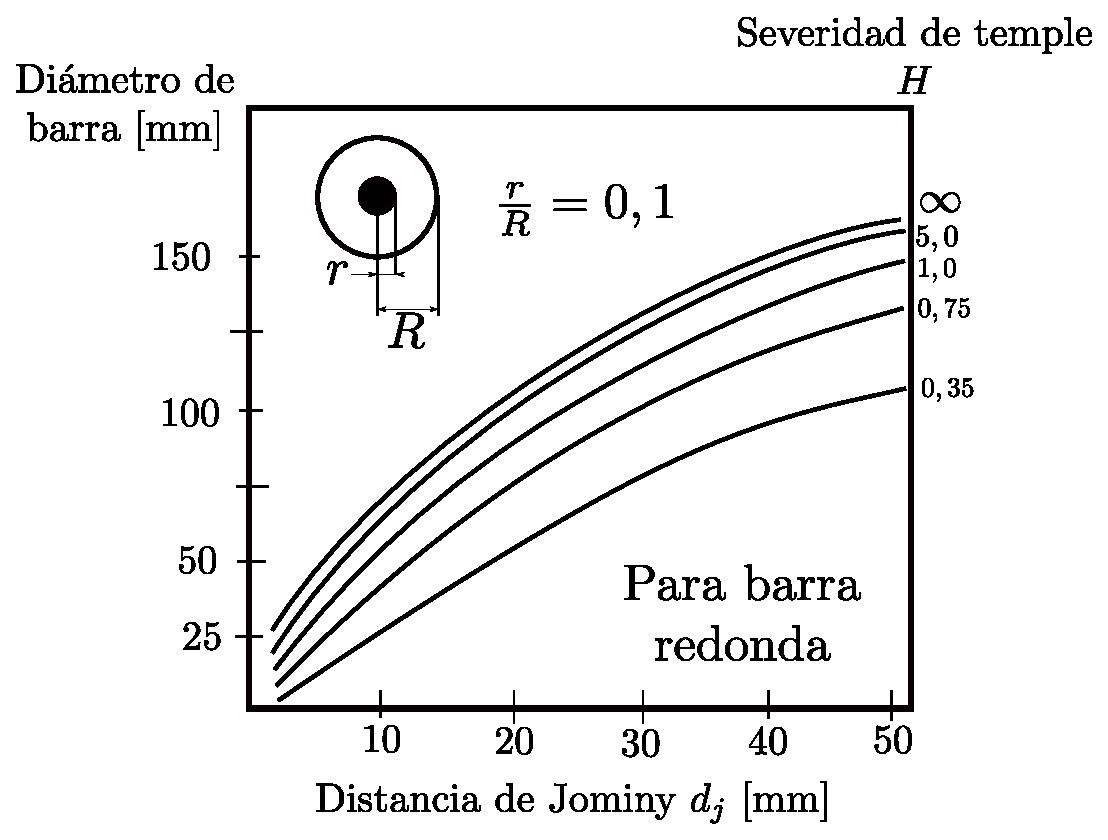
\includegraphics[width=0.8\textwidth]{fig/lamont.eps}
    \caption{Curva de Lamont para una barra redonda $\frac{r}{R}=0,1$.}
    \label{fig:lamont}
\end{figure}


\begin{figure}[htb!]
    \centering
    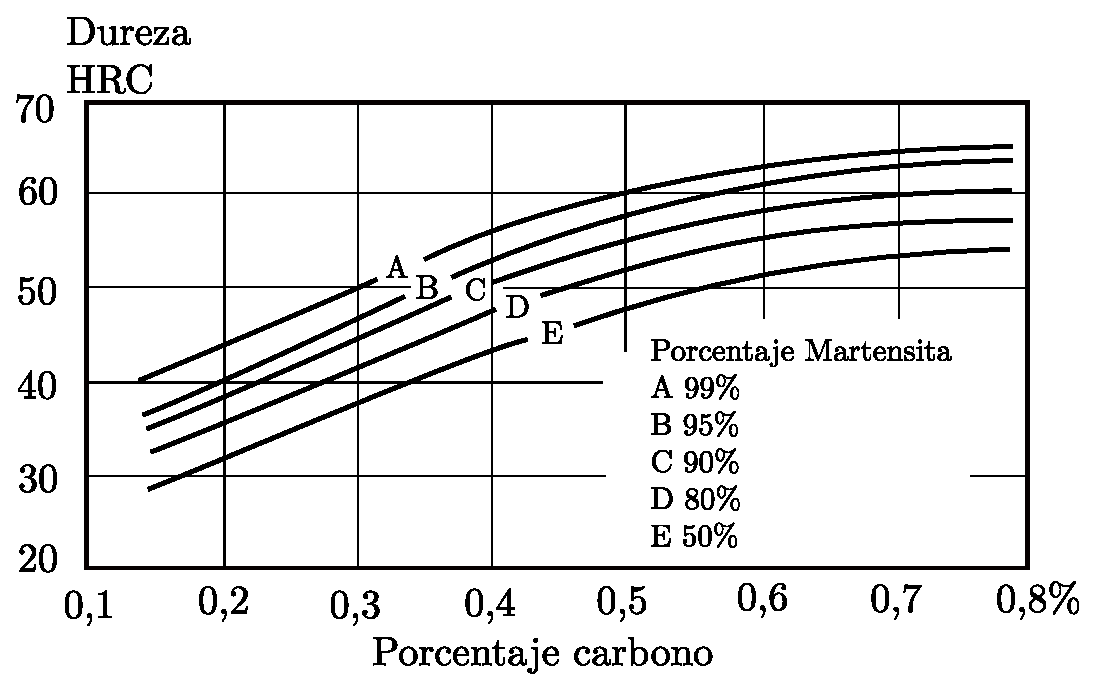
\includegraphics[width=0.8\textwidth]{fig/HRCdiag.eps}
    \caption{Tabla dureza Rockwell tipo `C' (HRC).}
    \label{fig:rockewell}
\end{figure}

\subsection{Temple de aceros hipereutectoides -- Austenita retenida}
\textbf{El temple de aceros hipereutectoides se debe hacer desde temperatura intercrítica.}

La austenita retenida es aquella que, luego del temple, no ha podido transformar a alta temperatura mediante transformaciones con difusión ni tampoco a baja temperatura a martensita. Es lo suficientemente estable a temperatura ambiente como para persistir en la estructura. Sin embargo existen algunas circunstancias que pueden transformarla.

\subsubsection{Variables que influyen en el porcentaje de austenita retenida}
\begin{itemize}
    \item \textbf{Composición química} de la austenita, principalmente \%C. Esto determina rango $M_s$--$M_f$
    \item \textbf{Homogeneidad} del acero (segregaciones)
    \item \textbf{Temperatura} del baño de temple
    \item \textbf{Interrupciones} en el temple. (cambio de medio enfriador)
    \item \textbf{Velocidad de enfriamiento} en el rango $M_s$--$M_f$
\end{itemize}

\subsubsection{Efectos de la austenita retenida}
\begin{itemize}
    \item Disminuye la dureza del temple (en altas proporciones)
    \item Produce \textbf{inestabilidad dimensional} a consecuencia de su posible transformación en servicio, ya sea transformación activada térmicamente a bainita o transformación a martensita activada por tension. En ambos casos la pieza \textbf{aumenta sus dimensiones}. Problema en piezas de tolerancias finas.
    \item Puede producir fallas por \textbf{astillado en filos} cuando transforma a martensita
    \item Cuando se encuentra en bajas proporciones contribuye en el \textbf{fenómeno de fragilización de la martensita revenida} en los aceros al C y de baja aleación.
    \item Si su proporción es baja, su distribución homogénea y fina, y dependiendo de su estabilidad, puede \textbf{aumentar la tenacidad} (aceros al Níquel para uso criogénico, fundiciones ADI, etc).
\end{itemize}

\subsubsection{Métodos para disminuir la cantidad de austenita retenida}
\begin{itemize}
    \item Revenido simple (solo efectivo en el caso de aceros al C y de baja aleación).
    \item Tratamiento criogénico (es caro, tiene altos riesgos de fisuración y requiere tratamientos intermedios de distensionado o revenidos).
    \item Revenidos múltiples (muy usados en el tratamiento de varias clases de aceros para herramientas). Este método puede combinarse con el anterior para mayor efectividad.
\end{itemize}


Proporciones usuales de austenita retenida luego de un temple correcto: 
\begin{itemize}
    \item Aceros al C y de baja aleación, de bajo y medio C: hasta 7\%.
    \item Aceros al C y de baja aleación, de alto C: 5 a 15\%.
    \item Aceros de alto C y alta aleación: 15 a 35\%.
\end{itemize}


\subsubsection{Temple hipercrítico}
Se obtiene principalmente martensita y una fracción alta de austenita retenida, reduciendo la dureza notablemente (puede sobrepasar 50\%). La templabilidad es alta pues todo el carbono y los aleantes están disueltos en la austenita inicial. Sin embargo, por las mismas razones $M_s$ y $M_f$ son bajas y se retiene mucha austenita. Suele ocurrir también con temples intercríticos cercanos a \Acm{}.

Hay riesgo de fisuración por temple por shock térmico.

\subsubsection{Temple intercrítico}
Compuesto principalmente por martensita, \cementita~ globular no disuelta a $T_A$ y una fracción menor de austenita retenida. Tiene templabilidad menor a la de un temple hipercrítico (pues la austenita es menos rica en carbono y aleantes), pero la $M_s$ y $M_f$ son más altas y no se retiene tanta austenita. Si la temperatura de austenización no es muy cercana a \Aone~ la dureza de temple en general es mayor que la del temple hipercrítico (menor \% austenita retenida). 

Si la temperatura es muy cercana a \Aone~ la falta de homogeneidad resultante en la austenita junto con el descenso de templabilidad y el menor porcentaje de carbono de la austenita pueden ser lo suficientemente importantes como para superar los efectos de reducción de la austenita retenida y la presencia de carburos. Debido a esto existe un \textbf{rango de temperaturas intercríticas óptimas} para cada acero hipereutectoide. Por arriba al rango se retendrá mucha austenita y por debajo caerá la templabilidad.

\begin{figure}[htb!]
    \centering
    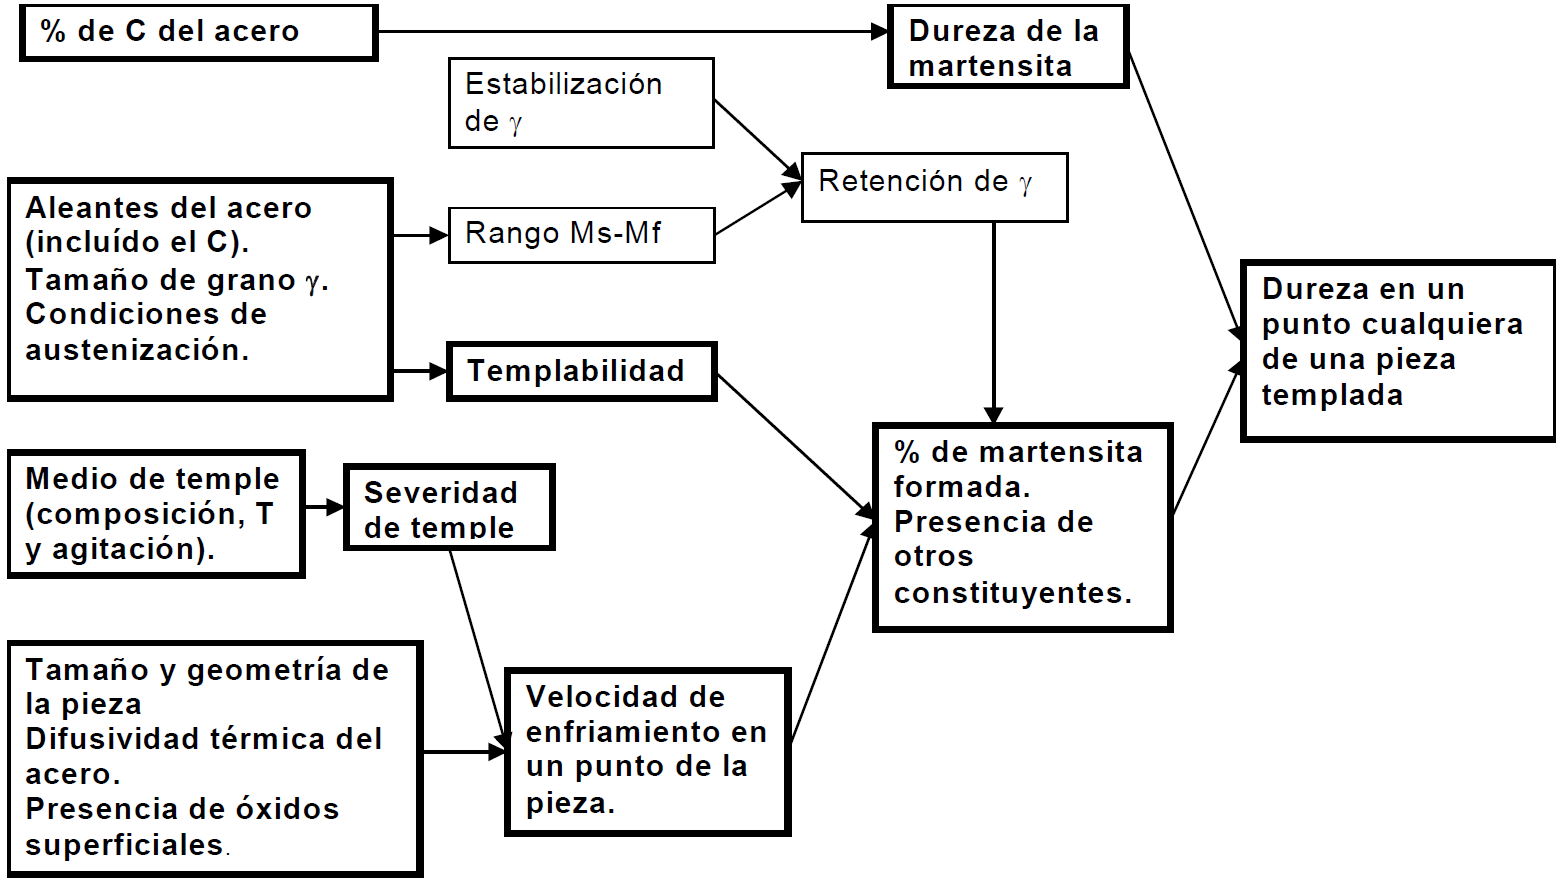
\includegraphics[width=.9\textwidth]{fig/flowdiagTemple.PNG}
    \caption{Diagrama de flujo para temple. Tener austenita no es para nada grave porque es potencialmente transformable a martensita.}
    \label{fig:flowdiagTemple}
\end{figure}

\section{Revenido}
Es un tratamiento subcrítico que se aplica luego del del temple con el objeto de 
\begin{itemize}
    \item Aumentar ductilidad y tenacidad de la martensita
    \item Lograr propiedades finales del acero
    \item Disminuir tensiones residuales
\end{itemize}

El ciclo térmico consiste en un \textbf{calentamiento} que puede tener varias etapas para evitar el choque térmico para el caso de aceros alta aleación/carbono. Se lleva el acero a la \textbf{temperatura de revenido} $T_R$ la cual varía de acuerdo a las propiedades deseadas ($T_R\in [150, \Aone )$\grad{}).  El \textbf{tiempo de revenido} es el tiempo que la pieza permanece a la temperatura de revenido. El tiempo varía del tamaño de la pieza y de las propiedades finales deseadas, aunque es de menor influencia que $T_R$ (tiempo de 30 min hasta 4 h para piezas tamaño medio). El \textbf{enfriamiento} se efectua en aire calmo excepto en dos casos: 
\begin{itemize}
    \item Cuando se desea disminuir las tensiones residuales se usa una \textbf{baja velocidad} de enfriamiento
    \item Para aceros susceptibles a la fragilización por revenido en cuyo caso se debe enfriar rápidamente en el rango de 580 a 400\grad.
\end{itemize}
\textbf{Revenidos multiples:} En ciertos casos se puede incluir un segundo o tercer calentamiento de $T_R$ igual o levemente diferente. Son usuales para aceros de medio y alto carbono/aleación.

\subsection{Etapas del revenido en aceros al carbono}

\begin{itemize}
    \item[Autorevenido] Ocurre durante el temple. Migración de átomos de carbono hacia zonas de alta densidad de defectos, formando un aglomerado de átomos carbono y/o precipitación de carburos durante el temple. Este fenómeno es más probable y completo a mayor $M_s$ del acero, es decir a bajo carbono\footnote{Ni bien se cruza $M_s$ las primeras martensitas que se forman pasan por un ``mini'' revenido. Este revenido preliminar es más pronunciado a mayor $M_s$.}
    \item[Etapa 1] (100 a 150\grad): Precipitación de carburo $\varepsilon$ ($\mathrm{Fe}_{2,5}\mathrm{C}$ estructura HCP). La precipitación de estas particulas submicroscópicas\footnote{Solo algunos nanometros.} es fina y homogenea causando endurecimiento por precipitación. Esta etapa no aparece en aceros de carbono menor a 0,2\% pues el autorevenido es suficientemente completo para que no haya fuerza impulsora para la precipitación de $\varepsilon$.
    \item[Etapa 2] ($>200\grad$): Transformación de la\textbf{ austenita retenida} a una estructura de ferrita y carburos
    \item [Etapa 3] (a partir de 250\grad): Disolución de los carburos $\varepsilon$ y \textbf{precipitación de cementita} \cementita. Desaparece la sobresaturación de carbono, la martensita deja de existir como una fase BCT y pasa a ser ferrita BCC cuando este problema se completa.
    \item[Etapa 4] (a partir de 300\grad): Coalescencia progresiva de las partículas de cementita. Fuerte descenso de dureza. A mayor temperatura y/o tiempo los carburos tienen mayor tamaño aunque su fracción en volumen permanece constante
\end{itemize}

Si bien no se las considera etapas, hay otros dos fenómenos que pueden
ocurrir a mayor temperatura de revenido.

A partir de los 400\grad~ ocurre la recuperación de las dislocaciones de la
martensita (formación de subgranos dentro de los listones).


A partir de los 600 \grad~ puede ocurrir la recristalización, los listones son
reemplazados por granos equiaxiales.

\hl{La estructura final de un revenido de alta temperatura en un acero al C
está compuesta por granos de ferrita pequeños y más o menos equiaxiales
y carburos finos (del orden de 0,1 micrometros) distribuidos uniformemente. Este
tipo de estructura combina una gran resistencia mecánica con una
muy alta tenacidad. Los carburos finos endurecen, pero su tamaño
pequeño, su forma esferoidal, y su distribución uniforme evitan que se
produzca un descenso muy grande en la tenacidad.}

\subsection[Resistencia al revenido]{Revenido de aceros de baja aleación (Resistencia al revenido)}

Ciertos aleantes participan en la formación de carburos (Cr, Mo, V, etc), sea cementitas aleadas (ortorrómbicas) o bien otros carburos aleados. Este tipo de carburos crece más lentamente que la cementita pues requiere la difusión de los aleantes (más lento que el carbono), así \textbf{ralentizando el revenido}. Por esta razón los aceros aleados se tienen que \textbf{revenir más tiempo o a mayor temperatura}.

También el agregado de aleantes agrega \textbf{complejidad a la secuencia de precipitación} de carburos, lo que puede producir un \textbf{máximo o pico de dureza} a altas temperaturas de revenido.

Los aleantes \textbf{retrasan} la descomposición de la austenita retenida y la recuperación de las dislocaciones de la martensita.



El resultado de todas estas influencia es que la dureza baja más lentamente durante el revenido de un acero con elementos\footnote{Cr, Mo, V, Ti, Nb, etc.} formadores de carburos que en un acero al carbono.

En ese sentido se dice que los aleantes aumentan la \hl{\textbf{resistencia al revenido}}. \cite{guille}

\subsection{Variación de propiedades mecánicas durante el revenido}
En aceros al carbono y de baja aleación al aumentar $T_R$ se produce un descenso en la resistencia mecánica y aumento en la ductilidad y tenacidad. 

El tiempo de revenido tiene menor efecto, aumentar $T_R$ 20\grad~ equivale a triplicar el tiempo de revenido.

Existen curvas ``maestras"{} que se representan en función del \textbf{parámetro de revenido}, teniendosé en cuenta el efecto conjunto de la temperatura y del tiempo de revenido. 

\subsection{Fenómenos de fragilización durante el revenido}
A pesar de la tendencia al aumento de la tenacidad durante el revenido,existen dos fenómenos de fragilización que deben tenerse en cuenta pues deterioran la tenacidad del acero:

\begin{itemize}
    \item \textbf{Fragilización de la martensita revenida}: Consiste en un descenso en la tenacidad durante el revenido en un rango de temperaturas intermedia.
    \item \textbf{Fragilización por revenido}: Consiste en un aumento de la temperatura de transición \Tdf. A pesar de su nombre no es un problema que ocurre en el revenido, pues requiere de tiempos de exposición muy prolongados en el rango de temperaturas de fragilización. Es más bien un problema en el servicio de componentes a alta temperatura.
\end{itemize}

\subsubsection{Fragilización de la martensita revenida}
Fenómeno de fragilización que ocurre durante el revenido de la martensita en el rango de 260 a 400\grad{}. Se produce en los tiempos usuales de un revenido (1h) y afecta tanto aceros al carbono como aleados. Si el revenido se realiza a $T_R>$400\grad el fenómeno no ocurre aunque la pieza sea sometida a temperaturas de fragilización durante su servicio. En este sentido se dice que es \textbf{irreversible}.

Efectos incluye un aumento de \Tdf~ y baja tenacidad. El modo de fractura frágil es intergranular solo en el caso de aceros de baja pureza\footnote{Recordemos que en aceros de baja pureza los carburos nuclean en los bordes de grano formando carburos a base de fósforo, Sb, Sn, As. Esto facilita la propagación de fisuras debido a la baja tenacidad de estos carburos.}, de otro modo es transgranular.

El fenómeno es lo suficientemente rápido como para tener influencia en cualquier revenido que se haga en el rango de susceptibilidad. En el caso en que se requiera alta tenacidad se debe evitar dicho rango. Esto impide obtener una tenacidad alta mediante temple y revenido cuando se requieren durezas altas.

\begin{figure}[htb!]
	\centering
	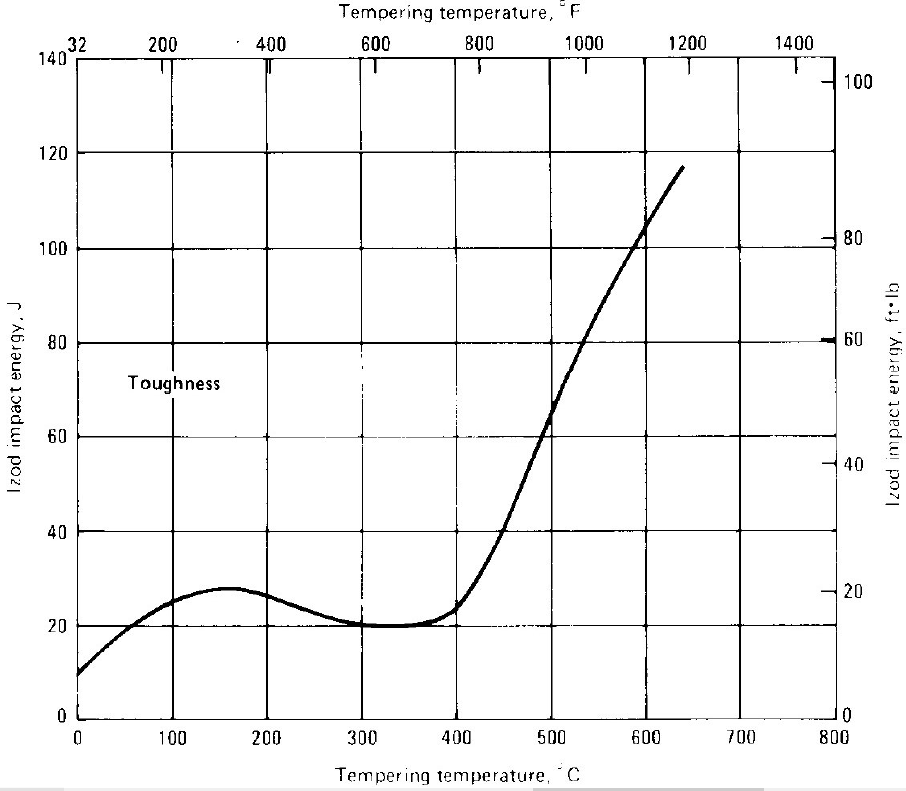
\includegraphics[width=7cm]{fig/fragilizacionPorRevenidoMartensita.png}\par \vspace{.4cm}
	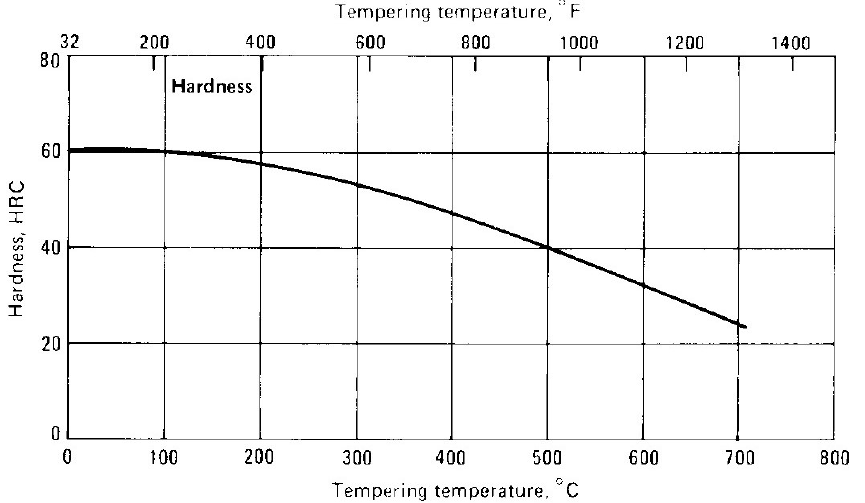
\includegraphics[width=7cm]{fig/fragilizacionPorRevenidoMartensitaDureza.png}
	\caption{Efecto de la \textbf{fragilización de la martensita revenida}. Gráfico de tenacidad y dureza para un acero 4140 revenido por una hora a varias temperaturas.}
\end{figure}


\textbf{Causas}: el descenso de la tenacidad está asociado a la precipitación de \cementita~ con una distribución y morfología particular durante el revenido. Estas características hacen que se reduzca fuertemente la energía absorbida durante el proceso de fractura. Las impurezas contribuyen por segregación hacia los bordes de grano, pero no son imprescindibles.

\subsection{Fragilización por revenido}
Fenómeno de fragilidad reversible que se produce cuando ciertos aceros se exponen prolongadamente o se enfrían lentamente en el rango de 400 a 580\grad{}. No debe confundirse con la fragilización de la martensita revenida (que se da a menor temperatura) o con la fragilización por creep (que se da a mayor temperatura).

Son susceptibles los aceros aleados de pureza comercial ($>0,6\%$ Mn) y los que tienen elevado contenido de impurezas: Sb, Sn, As, P. Ciertos aleantes aumentan la susceptibilidad, sobre todo si se encuentran combinados: Si, Mn, Cr-Ni, Cr-Mn. El molibdeno (Mo) y el tungsteno (W) bajan las susceptibilidad cuando se encuentran en pequeñas cantidades.

También es importante considerar este efecto para cuando se efectúan revenidos a grandes piezas a temperaturas mayores pero que se enfrían lentamente en el rango de fragilización. Se tiene que considerar que tal vez cierto componente esté trabajando dentro del rango de fragilización (rotores de turbinas de vapor de baja presión, algunos recipientes a presión).

Los \textbf{efectos incluye}
\begin{itemize}
    \item Aumento \Tdf~
    \item El modo de fractura frágil es intergranular
    \item Ciertos reactivos atacan los antiguos bordes de grano austeníticos
\end{itemize}

\textit{Teoría de la doble segregación} como \textbf{causa:} Las impurezas mencionadas segregan en los borde de grano austeníticos en el rango de temperaturas (400 a 580\grad) causando un descenso de la cohesión de los mismos. Este descenso eleva \Tdf~ y favorece la fisuración intergranular frente al modo de fractura frágil transgranular por clivaje. 

Esta teoría explica porque solo los aceros con ciertos aleantes son susceptibles y también porque la fisura avanza por los antiguos bordes de grano austeníticos y no por los borde de grano ferríticos.


\subsubsection{Medidas contra la fragilización por revenido}

\begin{itemize}
    \item Agregado de un bajo \% Mo retrasa fuertemente cinética de la fragilización
    \item Adecuada elección de los aleantes
    \item Reducción de impurezas
    \item Reducción de tamaño de grano austenítico, lo que no es tan fácil en piezas grandes
    \item En los casos de piezas que no trabajan en el rango de fragilización se \textbf{enfría rápidamente desde $T_R$}
    \item Se pueden recuperar piezas fragilizadas en servicio con un tratamiento de revenido $T_R>600$\grad.
    \item Monitoreo de la \Tdf~ en equipos que operen en el rango de fragilización. Técnicas no destructivas de monitoreo.
\end{itemize}

\subsection{Revenidos de alta y de baja temperatura}

La existencia del fenómeno de fragilización de la martensita revenida,
junto con la tendencia al aumento de la tenacidad que ocurre tanto a
temperaturas inferiores a las del rango de fragilización como a
temperaturas superiores al mismo, hace que existan dos rangos de
revenido bien definidos.
Los revenidos de \textbf{baja temperatura} (usualmente hasta unos 250 ºC) se
usan cuando es imprescindible retener una dureza muy alta en el acero,
lo cual implica un sacrificio de la tenacidad. El revenido en este rango
de temperaturas releva parcialmente las tensiones residuales del temple.
Los revenidos de \textbf{alta temperatura} (T>500 ºC) hacen que baje
sensiblemente la dureza de temple en el caso de los aceros al C y de baja
aleación, pero logran una excelente tenacidad con muy buena resistencia
mecánica.


\subsection{Revenido de microconsituyentes no martensiticos}

Al ser estructuras más estables, la velocidad de revenido de la perlita y
las bainitas es bastante inferior a la de la martensita.
En el revenido de la martensita, la mayor pérdida de dureza se da a causa
de la extracción del C en solución sólida sobresaturada y su precipitación
como carburo. En la perlita y la bainita esto no sucede.
En la bainita sólo ocurre un engrosamiento progresivo de los carburos y
una recuperación de las dislocaciones de la ferrita. Ambas cosas
conducen a una disminución de la dureza pero a un ritmo menor que en el
revenido de la martensita.
En el caso de la perlita el proceso de revenido es aún más lento, pues sólo
involucra la esferoidización progresiva de los carburos laminares. Tal
como ya se ha visto este proceso es muy lento.

La diferencia de velocidad con la que decae la dureza durante el revenido de las diferentes estructuras tiene la
importante consecuencia de
que el gradiente de durezas
que se produce luego del
temple, disminuye durante
el revenido, en especial para
altas temperaturas de
revenido.

\section{Martemperado}

Es un temple en dos etapas.
\begin{enumerate}
	\item El acero es enfriado hasta una temperatura ligeramente superior a $M_s$ y allí se mantiene hasta que homogenice su temperatura. Se mantiene 100\% contenido de austenita
	\item En la última etapa el acero es enfriado a una velocidad más lenta pasando por el rango $M_s$ y $M_f$.
	\item[Bis.] Se suele requerir un revenido posterior
\end{enumerate}
la temperatura a la cual se homogeneiza la pieza se denomina la temperatura de martemperado. El tiempo de mantención puede variar mucho (pocos segundos hasta 40 minutos)

No es la solución para adquirir más dureza o templabilidad, solo disminuye el riesgo de fisuración. Igual se requiere un revenido posterior. Se requiere una templabilidad mínima para poder aplicar martemperado y te limitan los espesores de las piezas a tratar.

\subsection{Ventajas}
\begin{itemize}
	\item Disminución de varios efectos incluyendo distorsión, tensiones residuales (macroscópicas) y riesgos de fisuración por temple. Es especialmente recomendado para aceros alto C y piezas esbeltas/complejas
	\item Mejoramiento de propiedades mecánicas respecto temple común (mayor ductilidad y tenacidad a igual resistencia mecánica)
	\item Permite realizar operaciones de enderezado luego de extraer la pieza del baño de martemperado y antes de que se transforme a martensita (aún sigue siendo austenita, asegura alta ductilidad y baja resistencia mecánica)
\end{itemize}



\subsection{Limitaciones}
\begin{itemize}
	\item El enfriamiento inicial es lento y requiere cierta templabilidad mínima. Como regla general solo aceros templables en aceite pueden ser martemperados
	\item Existe una limitación en espesores de las piezas a tratar (templabilidad mínima). Solo se pueden martemperar piezas de espesor grande si son de acero de alta templabilidad. Se puede agregar agua la medio o utilizar una temperatura de martemperado inferior a $M_s$ para aumentar el espesor permisible
\end{itemize}

\subsection{Aplicaciones del martemperado}
Se puede aplicar el martemperado a una gran variedad de piezas con geometría relativamente compleja y espesores no muy grandes hechas de aceros de baja aleación.

Se reduce el riesgo de fisuración en aceros de alto contenido de C y es de interés para piezas carburadas, y aceros de alta aleación donde es posible martemperar grandes secciones de piezas complejas. 



\section[Austemperado]{Austemperado (Austempering)}

Tratamiento isotérmico en el rango de la transformación bainítica. Se enfría el acero lo suficientemente rápido para evitar transformaciones de fases a temperaturas altas hasta llegar a una temperatura mayor a $M_s$ y se lo deja ahí hasta completar la transformación bainítica inferior.

No se austemperan aceros con transformación bainítica lenta ($>60$ minutos) ni los que no cumplan con la templabilidad mínima. La transformación ocurre alrededor de los 260\grad~ a 400\grad~ dependiendo del tipo de acero y nivel de resistencia deseado con un tiempo de mantención entre 5 a 60 minutos. Se suelen usar sales fundidas.

\subsection{Ventajas}
\begin{itemize}
    \item Se disminuye la distorsión, tensiones residuales y probabilidad de fisuración respecto temple y martemperado
    \item Tratamiento corto y económico para producir durezas en el rango 35 a 55 HRC pues no se requiere revenido posterior
    \item A diferencia del martemperado, el tiempo de permanencia en el baño de sales no afecta drásticamente las propiedades finales
    \item En el rango de durezas 45 a 55 HRC la bainita inferior posee aún mejor tenacidad que la martensita revenida a igualdad de durezas (esta tendencia se revierte en el rango HRC 35 a 45)
\end{itemize}

\subsection{Limitaciones}
No se puede aplicar a cualquier aceros por requerimientos de templabilidad. Las limitaciones son mayores que en el martemperado dado que el medio en el cual se enfría tiene una temperatura mayor a la del martemperado lo cual implica una velocidad de enfriamiento más lento.

El tiempo necesario varía dependiendo del acero. En ciertos casos el austemperado tarda mucho tiempo y no es viable economicamente. Además no se pueden alcanzar durezas superiores a 55 HRC, aún en aceros alto C.
% !TeX spellcheck = es_ES
% !TeX root = ../metalurgy.tex
\part{Aceros para construcción Mecánica}
Para fabricación de piezas de maquinaria. Cadena cinemática, transmisión de potencia, elementos roscados, herramientas manuales, industria automotriz, agrícola, aeronáutica, ferroviaria, etc.

Los \textbf{requerimientos de servicio} para un acero incluye propiedades mecánicas como $R_m$, $R_{p0,2}$, tenacidad, resistencia a la fatiga, resistencia al desgaste, resistencia a cargas de contacto. Luego se pueden exigir \textbf{caracteristicas de fabricación} como formabilidad, maquinabilidad y ductilidad. Los requerimientos de servicio y características de fabricación suelen obtenerse de tratamientos térmicos.

\section{Clasificación}

Existen varios tipos de clasificaciones de aceros para contrucción mecánica:

\subsection*{Según aleantes}
\begin{description}
	\item[Aceros al C] Más baratos, fácil fabricación y de menor templabilidad
	\item[Ac. de baja aleación] Buena templabilidad, menor severidad de temple requerida, buena maquinabilidad, buena resistencia al revenido
\end{description}


\subsection*{Clasificación por \%C}
\begin{description}
	\item[Bajo C ($<0,25\%$)] Para cementación/carburización (engranajes, árboles, cadenas)
	\item[Medio C ($0,25 \textrm{ a }0,5\%$)] Aceros para bonificado. Durezas $\approx 30$ a $40$ HRC
	\item[Bajo C ($>0,5\%$)] Máxima resistencia y dureza. Se usan bonificados, martemperados+revenidos, austemperados. Costo alto de fabricación de piezas por baja maquinabilidad y formabilidad.
\end{description}

\subsection*{Clasificación por templabilidad}
Puede ser baja, media o alta. El requerimiento de templabilidad va estar en función a la solicitación.

\begin{description}
	\item[Tracción/corte puro] 90\% mínimo de martensita en el centro. $R_{p0,2}>1200$ MPa. Bulones y tornillos de alto grado
	\item[Flexión/Torsión pura] 50\% martensita en el centro. Árboles, ejes y resortes
\end{description}

\section{Resistencia a la fatiga}
Se determina con un ensayo en la maquina de Moore (flexión rotativa $\sigma_m=0$;$\sigma_a = |\sigma_{\max}|$) definiéndose así las zonas de bajo y alto ciclado.

\subsection*{Como maximizar la resistencia a la fatiga}
En aceros al C de baja aleación con dureza 45 HRC se cumple que $R_f \approx 0,35 - 0,6R_u$ (Shigley toma $0,5R_u$). Esto es valido para una probeta lisa sin tensiones residuales bajo flexión alternativa.

Si se tiene una entalla
\[
q = \frac{k_f -1}{k_t - 1}
\]
$q$ indica cuanta tensión es relevada. $q=1 \Rightarrow$ muy sensible a la entalla.  Para maximizar la resistencia a la fatiga se necesita alta ductilidad y alta $R_m$. Se puede obtener por temple y revenido, o austemperado.

\section{Aceros al boro}
El boro promueve templabilidad a bajo costo en aceros de bajo y medio carbono. El boro (intersticial en la austenita) segrega a los bordes de grano retrasando la nucleación de ferrita proeutectoide. Se corren las curvas CCT a la derecha, ganándose mejor templabilidad.

El boro se puede encontrar en estos aceros en solución sólida, como óxido, nitruros, boruros. Se corre el peligro que al agregar demasiado boro vaya a formar un compuesto que no cumpla ser soluto.

\section{Aceros de corte libre}

Son aquellos con algunos elementos (P y S en general) que se usan cuando la pieza requiere mucho mecanizado y el costo es más importante que las propiedades finales. El azufre hace que se entrecorte la viruta y funcione como lubricante.  El fósforo en solución sólida hace que se fragilice la ferrita logrando viruta entrecortada. SAE 1100$\rightarrow$S; SAE 1200$\rightarrow$S,P.

% !TeX spellcheck = es_ES
% !TeX root = ../metalurgy.tex
\part{Aceros inoxidables}
Grupo de aceros de alta aleación diseñados para tener resistencia a la corrosión en un amplio rango de servicio (buena $R_m$ a altas temperaturas).

Las aplicaciones principales de estos aceros son en plantas generadoras de energía, centrales hidráulicas, plantas petroquímicas, industria farmacéutica, piezas de maquinas, arquitectura (decoración), aplicaciones marítimas.

\section{Corrosión}
Deterioro de un material por la acción química del medio que lo rodea. A excepción de los nobles, los metales son termodinámicamente inestables al contacto con el aire y forman óxidos. Si la reacción es ``lenta"{} (desde un punto de vista cinético) la corrosión puede llegar a aceptarse. Si es ``rápida"{} y limita la vida del componenta surgen problemas de costo y fiabilidad mecánica.

\subsection{Clasificación}
\begin{description}
	\item[Generalizada] A nivel macroscópico, la superficie es atacada uniformemente. Es predecible y controlable. Se puede prevenir si se diseña con un sobre-espesor uniforme. El daño es proporcional a la cantidad de material removido.
	\item[Localizada] Daño localizado progresa rápido. Resulta difícil predecir, controlar y detectar. El daño puede ser muy grande aunque la cantidad de material sea mínima. Es muy problemático. A continuación se tienen 4 tipos de corrosión localizada:
	\begin{description}
		\item[Picado/Pitting] Promovido por la presencia de iones $Cl^{-1}$, alta temperatura y baja velocidad de circulación del fluido. Si la capa pasivante se rompe localmente y no se forma rápido otra la corrosión avanza y se genera pozos en forma de túneles que pueden perforar el material en corto tiempo aumentando el riesgo de avance de fisura por fatiga.
		\item[Rendijas] Se da en zonas donde el fluido no llega a circular. Cuando se consume el oxigeno, se localiza la corrosión en la rendija. Evitable con buen diseño de pieza, reduciendo iones de cloro y reduciendo la temperatura
		\item[Bajo tensión] Puede dar lugar  fallas catastróficas a partir de fisuración provocada por la combinación del \textbf{medio} y \textbf{tensión de tracción}. Em general la fisura rompe por fractura frágil. Los aceros inoxidables austeníticos y martensiticos son los más susceptibles
		\item[Granular] Asociada a fenómeno de precipitación de carburos ricos en Cr en los bordes de grano de las microestructuras.
	\end{description}
\end{description}


\subsection{Pasividad}
La pasivación de un metal se refiere a la formación de una delgada capa de óxido al ser sometido a un diferencial de potencial ($\Delta V$) mayor al potencial de pasivación. Esta capa aísla al metal del medio y hace que disminuya la velocidad de corrosión en varios ordenes de magnitud. Para que sea efectiva la capa esta debe ser fina, continua, no porosa, insoluble en el medio, y debe poder regenerarse rápidamente al ser dañada (ralladura, mecanizado). 

Ek aluminio, por ejemplo, no es electronegativo pero es fuertemente pasivado. El hierro puede pasivarse pero a un alto $\Delta V$. La inclusión de cromo (Cr) en un 12\% o más hace que el metal pueda oxidarse fácil

\subsubsection*{Variables en la estabilidad de la capa pasivante}
\begin{description}
	\item[Composición química del acero] Factor principal es el contenido de Cr (12\% mínimo) para pasivar con soluciones acuosas neutras. En general la heterogeneidades (segregaciones, precip. de carburos) hacen que disminuya la estabilidad.
	\item[Composición del medio] Los inoxidables se pasivan solo cuando el medio es altamente oxidante (acuosos, $HNO_3$). La presencia de iones de halógenos es la principal razón por fallas. Estos iones desestabilizan y generan Pitting. Un medio básico (pH) es más estabilizante para una capa pasivante.
	\item[Variables operativas] En general, la resistencia a la corrosión disminuye con el aumento de la temperatura. La velocidad relativa entre el medio y la superficie afecta la formación de la capa. A mayor velocidad hay mayor aporte de $O_2$, aumentando la velocidad de oxidación.
	\item[Factores de diseño] La presencia de rendijas o alta rugosidad crean zonas que favorecen la oxidación localizada.
\end{description}

\section{Aceros inoxidables austeníticos}
Se trata del grupo de aceros inoxidables que mejor combina propiedades mecánicas y tecnologías con resistencia a la corrosión a precio razonable. Constituyen 70\% de la producción total de aceros inoxidables. 

La composición típica de un acero austenítico inoxidable:
\begin{description}
	\item[Cr] 16 a 30\%
	\item[Ni] 8 a 30\%
	\item[Mo] Hasta 4\%
	\item[Mn] $\approx$ 2\%
	\item[C] Menor de 0,1\%
\end{description}

\subsubsection*{Elección de gamágeno}
El Cr es un elemento alfágeno, entonces se necesita de un gamágeno para estabilizar la austenita a temperatura ambiente.
\begin{description}
	\item[C] Debe ser bajo porque favorece la precipitación de carburos de Cr, lo cual favorece la corrosión
	\item[N] No se usa ya que no estabiliza la austenita hasta bajas temperaturas
	\item[Mn] Se usa en casi todos los austeníticos pero no es el gamágeno principal. EStabiliza la austenita a temperatura ambiente pero no baja tanto $M_s$
	\item[Ni] Estabiliza austenita hasta bajas temperaturas. Baja la $M_s$ (reduciendo la formación de martensita, cosa indeseable), mejora la tenacidad y aumenta la resistencia a la corrosión. A mayor cantidad de Cr, Mo y otros alfágenos se requiere de mayor Ni para balancear.
\end{description}

\subsubsection*{Ventajas de la estructura FCC}
\begin{itemize}
	\item Ductilidad y baja $R_{p0,2}$. Alta capacidad de deformación en frío
	\item No hay transición dúctil frágil, alta tenacidad
	\item Resistencia al fenómeno del creep (fluencia a altas temperaturas)
	\item Los intersticiales tienen más solubilidad y menor difusividad. El Cr precipita más lento
	\item Amagnética
\end{itemize}

A temperatura ambiente un acero inoxidable austenítico contiene muy poca martensita por el $M_s$ bajo, poca ferrita y algunos carburos.

\subsubsection{Precipitación de carburos de Cromo}
El \%C disminuye la temperatura a la cual precipitan los carburos del Cromo y la ralentiza. Los carburos de Cromo nuclean en los borde de grano y bordes de maclas de la austenita. Alrededor de los carburos queda una zona empobrecida en Cr, lo cual lleva a la \textbf{sensibilización}.

La sensibilización da origen a la corrosión intergranular y ocurre frecuentemente en aceros austeníticos ya que cuando hay un proceso de alta temperatura el carbono se disuelve y re-precipita al enfriarse.


\bibliography{mybib}
\end{document}
